
% Default to the notebook output style

    


% Inherit from the specified cell style.




    
\documentclass[11pt]{article}

    
    
    \usepackage[T1]{fontenc}
    % Nicer default font (+ math font) than Computer Modern for most use cases
    \usepackage{mathpazo}

    % Basic figure setup, for now with no caption control since it's done
    % automatically by Pandoc (which extracts ![](path) syntax from Markdown).
    \usepackage{graphicx}
    % We will generate all images so they have a width \maxwidth. This means
    % that they will get their normal width if they fit onto the page, but
    % are scaled down if they would overflow the margins.
    \makeatletter
    \def\maxwidth{\ifdim\Gin@nat@width>\linewidth\linewidth
    \else\Gin@nat@width\fi}
    \makeatother
    \let\Oldincludegraphics\includegraphics
    % Set max figure width to be 80% of text width, for now hardcoded.
    \renewcommand{\includegraphics}[1]{\Oldincludegraphics[width=.8\maxwidth]{#1}}
    % Ensure that by default, figures have no caption (until we provide a
    % proper Figure object with a Caption API and a way to capture that
    % in the conversion process - todo).
    \usepackage{caption}
    \DeclareCaptionLabelFormat{nolabel}{}
    \captionsetup{labelformat=nolabel}

    \usepackage{adjustbox} % Used to constrain images to a maximum size 
    \usepackage{xcolor} % Allow colors to be defined
    \usepackage{enumerate} % Needed for markdown enumerations to work
    \usepackage{geometry} % Used to adjust the document margins
    \usepackage{amsmath} % Equations
    \usepackage{amssymb} % Equations
    \usepackage{textcomp} % defines textquotesingle
    % Hack from http://tex.stackexchange.com/a/47451/13684:
    \AtBeginDocument{%
        \def\PYZsq{\textquotesingle}% Upright quotes in Pygmentized code
    }
    \usepackage{upquote} % Upright quotes for verbatim code
    \usepackage{eurosym} % defines \euro
    \usepackage[mathletters]{ucs} % Extended unicode (utf-8) support
    \usepackage[utf8x]{inputenc} % Allow utf-8 characters in the tex document
    \usepackage{fancyvrb} % verbatim replacement that allows latex
    \usepackage{grffile} % extends the file name processing of package graphics 
                         % to support a larger range 
    % The hyperref package gives us a pdf with properly built
    % internal navigation ('pdf bookmarks' for the table of contents,
    % internal cross-reference links, web links for URLs, etc.)
    \usepackage{hyperref}
    \usepackage{longtable} % longtable support required by pandoc >1.10
    \usepackage{booktabs}  % table support for pandoc > 1.12.2
    \usepackage[inline]{enumitem} % IRkernel/repr support (it uses the enumerate* environment)
    \usepackage[normalem]{ulem} % ulem is needed to support strikethroughs (\sout)
                                % normalem makes italics be italics, not underlines
    

    
    
    % Colors for the hyperref package
    \definecolor{urlcolor}{rgb}{0,.145,.698}
    \definecolor{linkcolor}{rgb}{.71,0.21,0.01}
    \definecolor{citecolor}{rgb}{.12,.54,.11}

    % ANSI colors
    \definecolor{ansi-black}{HTML}{3E424D}
    \definecolor{ansi-black-intense}{HTML}{282C36}
    \definecolor{ansi-red}{HTML}{E75C58}
    \definecolor{ansi-red-intense}{HTML}{B22B31}
    \definecolor{ansi-green}{HTML}{00A250}
    \definecolor{ansi-green-intense}{HTML}{007427}
    \definecolor{ansi-yellow}{HTML}{DDB62B}
    \definecolor{ansi-yellow-intense}{HTML}{B27D12}
    \definecolor{ansi-blue}{HTML}{208FFB}
    \definecolor{ansi-blue-intense}{HTML}{0065CA}
    \definecolor{ansi-magenta}{HTML}{D160C4}
    \definecolor{ansi-magenta-intense}{HTML}{A03196}
    \definecolor{ansi-cyan}{HTML}{60C6C8}
    \definecolor{ansi-cyan-intense}{HTML}{258F8F}
    \definecolor{ansi-white}{HTML}{C5C1B4}
    \definecolor{ansi-white-intense}{HTML}{A1A6B2}

    % commands and environments needed by pandoc snippets
    % extracted from the output of `pandoc -s`
    \providecommand{\tightlist}{%
      \setlength{\itemsep}{0pt}\setlength{\parskip}{0pt}}
    \DefineVerbatimEnvironment{Highlighting}{Verbatim}{commandchars=\\\{\}}
    % Add ',fontsize=\small' for more characters per line
    \newenvironment{Shaded}{}{}
    \newcommand{\KeywordTok}[1]{\textcolor[rgb]{0.00,0.44,0.13}{\textbf{{#1}}}}
    \newcommand{\DataTypeTok}[1]{\textcolor[rgb]{0.56,0.13,0.00}{{#1}}}
    \newcommand{\DecValTok}[1]{\textcolor[rgb]{0.25,0.63,0.44}{{#1}}}
    \newcommand{\BaseNTok}[1]{\textcolor[rgb]{0.25,0.63,0.44}{{#1}}}
    \newcommand{\FloatTok}[1]{\textcolor[rgb]{0.25,0.63,0.44}{{#1}}}
    \newcommand{\CharTok}[1]{\textcolor[rgb]{0.25,0.44,0.63}{{#1}}}
    \newcommand{\StringTok}[1]{\textcolor[rgb]{0.25,0.44,0.63}{{#1}}}
    \newcommand{\CommentTok}[1]{\textcolor[rgb]{0.38,0.63,0.69}{\textit{{#1}}}}
    \newcommand{\OtherTok}[1]{\textcolor[rgb]{0.00,0.44,0.13}{{#1}}}
    \newcommand{\AlertTok}[1]{\textcolor[rgb]{1.00,0.00,0.00}{\textbf{{#1}}}}
    \newcommand{\FunctionTok}[1]{\textcolor[rgb]{0.02,0.16,0.49}{{#1}}}
    \newcommand{\RegionMarkerTok}[1]{{#1}}
    \newcommand{\ErrorTok}[1]{\textcolor[rgb]{1.00,0.00,0.00}{\textbf{{#1}}}}
    \newcommand{\NormalTok}[1]{{#1}}
    
    % Additional commands for more recent versions of Pandoc
    \newcommand{\ConstantTok}[1]{\textcolor[rgb]{0.53,0.00,0.00}{{#1}}}
    \newcommand{\SpecialCharTok}[1]{\textcolor[rgb]{0.25,0.44,0.63}{{#1}}}
    \newcommand{\VerbatimStringTok}[1]{\textcolor[rgb]{0.25,0.44,0.63}{{#1}}}
    \newcommand{\SpecialStringTok}[1]{\textcolor[rgb]{0.73,0.40,0.53}{{#1}}}
    \newcommand{\ImportTok}[1]{{#1}}
    \newcommand{\DocumentationTok}[1]{\textcolor[rgb]{0.73,0.13,0.13}{\textit{{#1}}}}
    \newcommand{\AnnotationTok}[1]{\textcolor[rgb]{0.38,0.63,0.69}{\textbf{\textit{{#1}}}}}
    \newcommand{\CommentVarTok}[1]{\textcolor[rgb]{0.38,0.63,0.69}{\textbf{\textit{{#1}}}}}
    \newcommand{\VariableTok}[1]{\textcolor[rgb]{0.10,0.09,0.49}{{#1}}}
    \newcommand{\ControlFlowTok}[1]{\textcolor[rgb]{0.00,0.44,0.13}{\textbf{{#1}}}}
    \newcommand{\OperatorTok}[1]{\textcolor[rgb]{0.40,0.40,0.40}{{#1}}}
    \newcommand{\BuiltInTok}[1]{{#1}}
    \newcommand{\ExtensionTok}[1]{{#1}}
    \newcommand{\PreprocessorTok}[1]{\textcolor[rgb]{0.74,0.48,0.00}{{#1}}}
    \newcommand{\AttributeTok}[1]{\textcolor[rgb]{0.49,0.56,0.16}{{#1}}}
    \newcommand{\InformationTok}[1]{\textcolor[rgb]{0.38,0.63,0.69}{\textbf{\textit{{#1}}}}}
    \newcommand{\WarningTok}[1]{\textcolor[rgb]{0.38,0.63,0.69}{\textbf{\textit{{#1}}}}}
    
    \usepackage{relsize}
    
    % Define a nice break command that doesn't care if a line doesn't already
    % exist.
    \def\br{\hspace*{\fill} \\* }
    % Math Jax compatability definitions
    \def\gt{>}
    \def\lt{<}
    % Document parameters
    \title{Lunak \\ [0.2em]\smaller{A Feed-forward Artificial Neural Network Implemented in Python}}
    \author{Felix Limanta—13515065 \\ Holy Lovenia—13515113 \\ Agus Gunawan—13515143}
    
    
    

    % Pygments definitions
    
\makeatletter
\def\PY@reset{\let\PY@it=\relax \let\PY@bf=\relax%
    \let\PY@ul=\relax \let\PY@tc=\relax%
    \let\PY@bc=\relax \let\PY@ff=\relax}
\def\PY@tok#1{\csname PY@tok@#1\endcsname}
\def\PY@toks#1+{\ifx\relax#1\empty\else%
    \PY@tok{#1}\expandafter\PY@toks\fi}
\def\PY@do#1{\PY@bc{\PY@tc{\PY@ul{%
    \PY@it{\PY@bf{\PY@ff{#1}}}}}}}
\def\PY#1#2{\PY@reset\PY@toks#1+\relax+\PY@do{#2}}

\expandafter\def\csname PY@tok@w\endcsname{\def\PY@tc##1{\textcolor[rgb]{0.73,0.73,0.73}{##1}}}
\expandafter\def\csname PY@tok@c\endcsname{\let\PY@it=\textit\def\PY@tc##1{\textcolor[rgb]{0.25,0.50,0.50}{##1}}}
\expandafter\def\csname PY@tok@cp\endcsname{\def\PY@tc##1{\textcolor[rgb]{0.74,0.48,0.00}{##1}}}
\expandafter\def\csname PY@tok@k\endcsname{\let\PY@bf=\textbf\def\PY@tc##1{\textcolor[rgb]{0.00,0.50,0.00}{##1}}}
\expandafter\def\csname PY@tok@kp\endcsname{\def\PY@tc##1{\textcolor[rgb]{0.00,0.50,0.00}{##1}}}
\expandafter\def\csname PY@tok@kt\endcsname{\def\PY@tc##1{\textcolor[rgb]{0.69,0.00,0.25}{##1}}}
\expandafter\def\csname PY@tok@o\endcsname{\def\PY@tc##1{\textcolor[rgb]{0.40,0.40,0.40}{##1}}}
\expandafter\def\csname PY@tok@ow\endcsname{\let\PY@bf=\textbf\def\PY@tc##1{\textcolor[rgb]{0.67,0.13,1.00}{##1}}}
\expandafter\def\csname PY@tok@nb\endcsname{\def\PY@tc##1{\textcolor[rgb]{0.00,0.50,0.00}{##1}}}
\expandafter\def\csname PY@tok@nf\endcsname{\def\PY@tc##1{\textcolor[rgb]{0.00,0.00,1.00}{##1}}}
\expandafter\def\csname PY@tok@nc\endcsname{\let\PY@bf=\textbf\def\PY@tc##1{\textcolor[rgb]{0.00,0.00,1.00}{##1}}}
\expandafter\def\csname PY@tok@nn\endcsname{\let\PY@bf=\textbf\def\PY@tc##1{\textcolor[rgb]{0.00,0.00,1.00}{##1}}}
\expandafter\def\csname PY@tok@ne\endcsname{\let\PY@bf=\textbf\def\PY@tc##1{\textcolor[rgb]{0.82,0.25,0.23}{##1}}}
\expandafter\def\csname PY@tok@nv\endcsname{\def\PY@tc##1{\textcolor[rgb]{0.10,0.09,0.49}{##1}}}
\expandafter\def\csname PY@tok@no\endcsname{\def\PY@tc##1{\textcolor[rgb]{0.53,0.00,0.00}{##1}}}
\expandafter\def\csname PY@tok@nl\endcsname{\def\PY@tc##1{\textcolor[rgb]{0.63,0.63,0.00}{##1}}}
\expandafter\def\csname PY@tok@ni\endcsname{\let\PY@bf=\textbf\def\PY@tc##1{\textcolor[rgb]{0.60,0.60,0.60}{##1}}}
\expandafter\def\csname PY@tok@na\endcsname{\def\PY@tc##1{\textcolor[rgb]{0.49,0.56,0.16}{##1}}}
\expandafter\def\csname PY@tok@nt\endcsname{\let\PY@bf=\textbf\def\PY@tc##1{\textcolor[rgb]{0.00,0.50,0.00}{##1}}}
\expandafter\def\csname PY@tok@nd\endcsname{\def\PY@tc##1{\textcolor[rgb]{0.67,0.13,1.00}{##1}}}
\expandafter\def\csname PY@tok@s\endcsname{\def\PY@tc##1{\textcolor[rgb]{0.73,0.13,0.13}{##1}}}
\expandafter\def\csname PY@tok@sd\endcsname{\let\PY@it=\textit\def\PY@tc##1{\textcolor[rgb]{0.73,0.13,0.13}{##1}}}
\expandafter\def\csname PY@tok@si\endcsname{\let\PY@bf=\textbf\def\PY@tc##1{\textcolor[rgb]{0.73,0.40,0.53}{##1}}}
\expandafter\def\csname PY@tok@se\endcsname{\let\PY@bf=\textbf\def\PY@tc##1{\textcolor[rgb]{0.73,0.40,0.13}{##1}}}
\expandafter\def\csname PY@tok@sr\endcsname{\def\PY@tc##1{\textcolor[rgb]{0.73,0.40,0.53}{##1}}}
\expandafter\def\csname PY@tok@ss\endcsname{\def\PY@tc##1{\textcolor[rgb]{0.10,0.09,0.49}{##1}}}
\expandafter\def\csname PY@tok@sx\endcsname{\def\PY@tc##1{\textcolor[rgb]{0.00,0.50,0.00}{##1}}}
\expandafter\def\csname PY@tok@m\endcsname{\def\PY@tc##1{\textcolor[rgb]{0.40,0.40,0.40}{##1}}}
\expandafter\def\csname PY@tok@gh\endcsname{\let\PY@bf=\textbf\def\PY@tc##1{\textcolor[rgb]{0.00,0.00,0.50}{##1}}}
\expandafter\def\csname PY@tok@gu\endcsname{\let\PY@bf=\textbf\def\PY@tc##1{\textcolor[rgb]{0.50,0.00,0.50}{##1}}}
\expandafter\def\csname PY@tok@gd\endcsname{\def\PY@tc##1{\textcolor[rgb]{0.63,0.00,0.00}{##1}}}
\expandafter\def\csname PY@tok@gi\endcsname{\def\PY@tc##1{\textcolor[rgb]{0.00,0.63,0.00}{##1}}}
\expandafter\def\csname PY@tok@gr\endcsname{\def\PY@tc##1{\textcolor[rgb]{1.00,0.00,0.00}{##1}}}
\expandafter\def\csname PY@tok@ge\endcsname{\let\PY@it=\textit}
\expandafter\def\csname PY@tok@gs\endcsname{\let\PY@bf=\textbf}
\expandafter\def\csname PY@tok@gp\endcsname{\let\PY@bf=\textbf\def\PY@tc##1{\textcolor[rgb]{0.00,0.00,0.50}{##1}}}
\expandafter\def\csname PY@tok@go\endcsname{\def\PY@tc##1{\textcolor[rgb]{0.53,0.53,0.53}{##1}}}
\expandafter\def\csname PY@tok@gt\endcsname{\def\PY@tc##1{\textcolor[rgb]{0.00,0.27,0.87}{##1}}}
\expandafter\def\csname PY@tok@err\endcsname{\def\PY@bc##1{\setlength{\fboxsep}{0pt}\fcolorbox[rgb]{1.00,0.00,0.00}{1,1,1}{\strut ##1}}}
\expandafter\def\csname PY@tok@kc\endcsname{\let\PY@bf=\textbf\def\PY@tc##1{\textcolor[rgb]{0.00,0.50,0.00}{##1}}}
\expandafter\def\csname PY@tok@kd\endcsname{\let\PY@bf=\textbf\def\PY@tc##1{\textcolor[rgb]{0.00,0.50,0.00}{##1}}}
\expandafter\def\csname PY@tok@kn\endcsname{\let\PY@bf=\textbf\def\PY@tc##1{\textcolor[rgb]{0.00,0.50,0.00}{##1}}}
\expandafter\def\csname PY@tok@kr\endcsname{\let\PY@bf=\textbf\def\PY@tc##1{\textcolor[rgb]{0.00,0.50,0.00}{##1}}}
\expandafter\def\csname PY@tok@bp\endcsname{\def\PY@tc##1{\textcolor[rgb]{0.00,0.50,0.00}{##1}}}
\expandafter\def\csname PY@tok@fm\endcsname{\def\PY@tc##1{\textcolor[rgb]{0.00,0.00,1.00}{##1}}}
\expandafter\def\csname PY@tok@vc\endcsname{\def\PY@tc##1{\textcolor[rgb]{0.10,0.09,0.49}{##1}}}
\expandafter\def\csname PY@tok@vg\endcsname{\def\PY@tc##1{\textcolor[rgb]{0.10,0.09,0.49}{##1}}}
\expandafter\def\csname PY@tok@vi\endcsname{\def\PY@tc##1{\textcolor[rgb]{0.10,0.09,0.49}{##1}}}
\expandafter\def\csname PY@tok@vm\endcsname{\def\PY@tc##1{\textcolor[rgb]{0.10,0.09,0.49}{##1}}}
\expandafter\def\csname PY@tok@sa\endcsname{\def\PY@tc##1{\textcolor[rgb]{0.73,0.13,0.13}{##1}}}
\expandafter\def\csname PY@tok@sb\endcsname{\def\PY@tc##1{\textcolor[rgb]{0.73,0.13,0.13}{##1}}}
\expandafter\def\csname PY@tok@sc\endcsname{\def\PY@tc##1{\textcolor[rgb]{0.73,0.13,0.13}{##1}}}
\expandafter\def\csname PY@tok@dl\endcsname{\def\PY@tc##1{\textcolor[rgb]{0.73,0.13,0.13}{##1}}}
\expandafter\def\csname PY@tok@s2\endcsname{\def\PY@tc##1{\textcolor[rgb]{0.73,0.13,0.13}{##1}}}
\expandafter\def\csname PY@tok@sh\endcsname{\def\PY@tc##1{\textcolor[rgb]{0.73,0.13,0.13}{##1}}}
\expandafter\def\csname PY@tok@s1\endcsname{\def\PY@tc##1{\textcolor[rgb]{0.73,0.13,0.13}{##1}}}
\expandafter\def\csname PY@tok@mb\endcsname{\def\PY@tc##1{\textcolor[rgb]{0.40,0.40,0.40}{##1}}}
\expandafter\def\csname PY@tok@mf\endcsname{\def\PY@tc##1{\textcolor[rgb]{0.40,0.40,0.40}{##1}}}
\expandafter\def\csname PY@tok@mh\endcsname{\def\PY@tc##1{\textcolor[rgb]{0.40,0.40,0.40}{##1}}}
\expandafter\def\csname PY@tok@mi\endcsname{\def\PY@tc##1{\textcolor[rgb]{0.40,0.40,0.40}{##1}}}
\expandafter\def\csname PY@tok@il\endcsname{\def\PY@tc##1{\textcolor[rgb]{0.40,0.40,0.40}{##1}}}
\expandafter\def\csname PY@tok@mo\endcsname{\def\PY@tc##1{\textcolor[rgb]{0.40,0.40,0.40}{##1}}}
\expandafter\def\csname PY@tok@ch\endcsname{\let\PY@it=\textit\def\PY@tc##1{\textcolor[rgb]{0.25,0.50,0.50}{##1}}}
\expandafter\def\csname PY@tok@cm\endcsname{\let\PY@it=\textit\def\PY@tc##1{\textcolor[rgb]{0.25,0.50,0.50}{##1}}}
\expandafter\def\csname PY@tok@cpf\endcsname{\let\PY@it=\textit\def\PY@tc##1{\textcolor[rgb]{0.25,0.50,0.50}{##1}}}
\expandafter\def\csname PY@tok@c1\endcsname{\let\PY@it=\textit\def\PY@tc##1{\textcolor[rgb]{0.25,0.50,0.50}{##1}}}
\expandafter\def\csname PY@tok@cs\endcsname{\let\PY@it=\textit\def\PY@tc##1{\textcolor[rgb]{0.25,0.50,0.50}{##1}}}

\def\PYZbs{\char`\\}
\def\PYZus{\char`\_}
\def\PYZob{\char`\{}
\def\PYZcb{\char`\}}
\def\PYZca{\char`\^}
\def\PYZam{\char`\&}
\def\PYZlt{\char`\<}
\def\PYZgt{\char`\>}
\def\PYZsh{\char`\#}
\def\PYZpc{\char`\%}
\def\PYZdl{\char`\$}
\def\PYZhy{\char`\-}
\def\PYZsq{\char`\'}
\def\PYZdq{\char`\"}
\def\PYZti{\char`\~}
% for compatibility with earlier versions
\def\PYZat{@}
\def\PYZlb{[}
\def\PYZrb{]}
\makeatother


    % Exact colors from NB
    \definecolor{incolor}{rgb}{0.0, 0.0, 0.5}
    \definecolor{outcolor}{rgb}{0.545, 0.0, 0.0}



    
    % Prevent overflowing lines due to hard-to-break entities
    \sloppy 
    % Setup hyperref package
    \hypersetup{
      breaklinks=true,  % so long urls are correctly broken across lines
      colorlinks=true,
      urlcolor=urlcolor,
      linkcolor=linkcolor,
      citecolor=citecolor,
      }
    % Slightly bigger margins than the latex defaults
    
    \geometry{verbose,tmargin=1in,bmargin=1in,lmargin=1in,rmargin=1in}
    
    

    \begin{document}
    
    
    \maketitle
    
    
    \hypertarget{introduction}{%
\section{Introduction}\label{introduction}}

An artificial neural network (ANN) is made of interconnected layers of
nodes, emulating the structures and functions of neurons in human brain.

Normally, connections between the nodes (neurons) are called edges.
These edges are associated with weights, which adjusts themselves during
the learning process.

\begin{figure}[h]
\centering
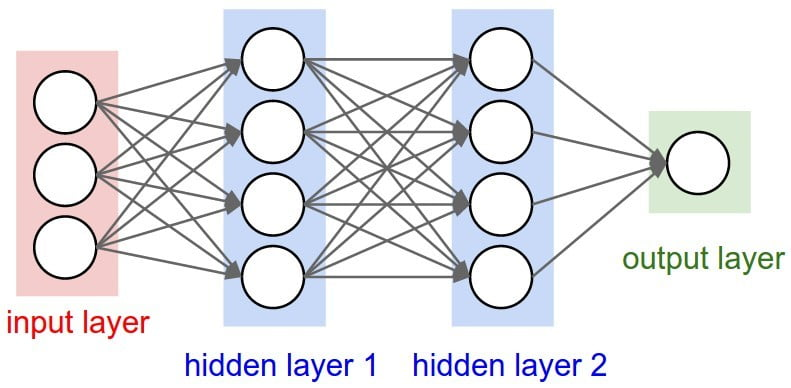
\includegraphics{img/artificial_neural_network_1-791x388.jpg}
\caption{Artificial neural network}
\end{figure}

Nodes are typically grouped into specific layers. Different layers
perform different transformations on their inputs. The first layer is
regarded as input layer; the last is output layer. The output layer
represents the final outputs of the network their corresponding
predicted classes. Between the two layers, hidden layers may be present
to process and transform the inputs by applying an activation function,
then produce results according to the needs of output layer.

The disconnected nodes in the network are called as bias nodes, which
are useful to shift the activation function into a desired direction.
Below is an example of network with the presence of bias nodes.

\begin{figure}[h]
\centering
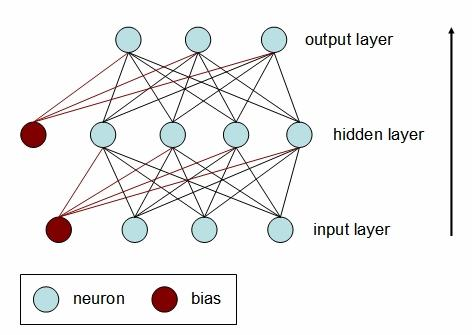
\includegraphics{img/mlpdiagram.jpg}
\caption{Network with bias}
\end{figure}

    \hypertarget{implementing-an-artificial-neural-network}{%
\section{Implementing an Artificial Neural
Network}\label{implementing-an-artificial-neural-network}}

We introduce Lunak, a simple feed-forward neural network implementation
in Python. The entire source code for Lunak is contained within this
report and shall be shown in the following subsections.

    \begin{Verbatim}[commandchars=\\\{\}]
{\color{incolor}In [{\color{incolor}1}]:} \PY{k+kn}{from} \PY{n+nn}{random} \PY{k}{import} \PY{n}{random}\PY{p}{,} \PY{n}{randint}
        \PY{k+kn}{from} \PY{n+nn}{sklearn}\PY{n+nn}{.}\PY{n+nn}{metrics} \PY{k}{import} \PY{n}{confusion\PYZus{}matrix}\PY{p}{,} \PY{n}{mean\PYZus{}squared\PYZus{}error}
        \PY{k+kn}{from} \PY{n+nn}{sklearn}\PY{n+nn}{.}\PY{n+nn}{model\PYZus{}selection} \PY{k}{import} \PY{n}{train\PYZus{}test\PYZus{}split}
        \PY{k+kn}{from} \PY{n+nn}{tqdm} \PY{k}{import} \PY{n}{tqdm}\PY{p}{,} \PY{n}{tnrange}
        
        \PY{k+kn}{import} \PY{n+nn}{math}
        \PY{k+kn}{import} \PY{n+nn}{numpy} \PY{k}{as} \PY{n+nn}{np}
        \PY{k+kn}{import} \PY{n+nn}{pandas} \PY{k}{as} \PY{n+nn}{pd}
\end{Verbatim}


    \hypertarget{implementing-the-layers}{%
\subsection{Implementing the layers}\label{implementing-the-layers}}

    We implement the \texttt{LunakDense} class to represent our hidden layer
and output layer. The parameters for this class are as follows.

\begin{enumerate}
\def\labelenumi{\arabic{enumi}.}
\tightlist
\item
  \texttt{units}: \texttt{int}, the number of nodes in the layer
\item
  \texttt{activation}:
  \texttt{\textquotesingle{}sigmoid\textquotesingle{}}, activation
  function
\item
  \texttt{input\_dim}: \texttt{int}, dimension of the input (e.g.~2D,
  3D, \ldots{})
\item
  \texttt{init}:
  \texttt{\textquotesingle{}uniform\textquotesingle{},\ \textquotesingle{}random\textquotesingle{}},
  type of distribution for the initial weight matrix
\item
  \texttt{use\_bias}: \texttt{boolean}, whether there will be bias node
  present or not (default=\texttt{False})
\item
  \texttt{seed}: \texttt{int}, the number of random seed
  (default=\texttt{None})
\end{enumerate}

    The layer transforms input \(p_j(t)\) to neuron \(j\) from the outputs
\(o_i(t)\) of predecessor neurons and bias \(w_{0j}\) according to the
following propagation function.

\[p_j(t) = \sum_{i} o_i(t) w_{ij} + w_{0j}\]

    \begin{Verbatim}[commandchars=\\\{\}]
{\color{incolor}In [{\color{incolor}2}]:} \PY{k}{class} \PY{n+nc}{LunakDense}\PY{p}{:}
            \PY{k}{def} \PY{n+nf}{\PYZus{}\PYZus{}init\PYZus{}\PYZus{}}\PY{p}{(}\PY{n+nb+bp}{self}\PY{p}{,} \PY{n}{units}\PY{p}{,} \PY{n}{activation}\PY{p}{,}
                         \PY{n}{input\PYZus{}dim}\PY{p}{,} \PY{n}{init}\PY{p}{,} \PY{n}{use\PYZus{}bias}\PY{o}{=}\PY{k+kc}{False}\PY{p}{,} \PY{n}{seed}\PY{o}{=}\PY{k+kc}{None}\PY{p}{)}\PY{p}{:}
                \PY{n+nb+bp}{self}\PY{o}{.}\PY{n}{units} \PY{o}{=} \PY{n}{units}
                \PY{n+nb+bp}{self}\PY{o}{.}\PY{n}{input\PYZus{}dim} \PY{o}{=} \PY{n}{input\PYZus{}dim}
                
                \PY{k}{if} \PY{n}{activation} \PY{o}{==} \PY{l+s+s1}{\PYZsq{}}\PY{l+s+s1}{sigmoid}\PY{l+s+s1}{\PYZsq{}}\PY{p}{:}
                    \PY{n+nb+bp}{self}\PY{o}{.}\PY{n}{activation\PYZus{}function} \PY{o}{=} \PY{n+nb+bp}{self}\PY{o}{.}\PY{n}{sigmoid}
                \PY{k}{else}\PY{p}{:}
                    \PY{n+nb}{print}\PY{p}{(}\PY{l+s+s1}{\PYZsq{}}\PY{l+s+s1}{Activation function not supported}\PY{l+s+s1}{\PYZsq{}}\PY{p}{)}
                
                \PY{n}{np}\PY{o}{.}\PY{n}{random}\PY{o}{.}\PY{n}{seed}\PY{p}{(}\PY{n}{seed}\PY{p}{)}
                
                \PY{k}{if} \PY{n}{init} \PY{o}{==} \PY{l+s+s1}{\PYZsq{}}\PY{l+s+s1}{uniform}\PY{l+s+s1}{\PYZsq{}}\PY{p}{:}
                    \PY{n+nb+bp}{self}\PY{o}{.}\PY{n}{weight\PYZus{}matrix} \PY{o}{=} \PY{n}{np}\PY{o}{.}\PY{n}{random}\PY{o}{.}\PY{n}{uniform}\PY{p}{(}\PY{o}{\PYZhy{}}\PY{l+m+mf}{0.05}\PY{p}{,} \PY{l+m+mf}{0.05}\PY{p}{,}
                                                           \PY{n}{size}\PY{o}{=}\PY{p}{(}\PY{n+nb+bp}{self}\PY{o}{.}\PY{n}{units}\PY{p}{,} \PY{n}{input\PYZus{}dim}\PY{p}{)}\PY{p}{)} 
                \PY{k}{elif} \PY{n}{init} \PY{o}{==} \PY{l+s+s1}{\PYZsq{}}\PY{l+s+s1}{random}\PY{l+s+s1}{\PYZsq{}}\PY{p}{:}
                    \PY{n+nb+bp}{self}\PY{o}{.}\PY{n}{weight\PYZus{}matrix} \PY{o}{=} \PY{n}{np}\PY{o}{.}\PY{n}{random}\PY{o}{.}\PY{n}{random}\PY{p}{(}\PY{n}{size}\PY{o}{=}\PY{p}{(}\PY{n+nb+bp}{self}\PY{o}{.}\PY{n}{units}\PY{p}{,} \PY{n}{input\PYZus{}dim}\PY{p}{)}\PY{p}{)}
                \PY{k}{else}\PY{p}{:}
                    \PY{n+nb}{print}\PY{p}{(}\PY{l+s+s1}{\PYZsq{}}\PY{l+s+s1}{Init function not supported}\PY{l+s+s1}{\PYZsq{}}\PY{p}{)}
                
                \PY{n+nb+bp}{self}\PY{o}{.}\PY{n}{delta\PYZus{}weight\PYZus{}matrix\PYZus{}before} \PY{o}{=} \PY{n}{np}\PY{o}{.}\PY{n}{zeros}\PY{p}{(}\PY{p}{(}\PY{n+nb+bp}{self}\PY{o}{.}\PY{n}{units}\PY{p}{,} \PY{n}{input\PYZus{}dim}\PY{p}{)}\PY{p}{)}
                \PY{n+nb+bp}{self}\PY{o}{.}\PY{n}{delta\PYZus{}weight\PYZus{}matrix} \PY{o}{=} \PY{n}{np}\PY{o}{.}\PY{n}{zeros}\PY{p}{(}\PY{p}{(}\PY{n+nb+bp}{self}\PY{o}{.}\PY{n}{units}\PY{p}{,} \PY{n}{input\PYZus{}dim}\PY{p}{)}\PY{p}{)}
                
                \PY{n+nb+bp}{self}\PY{o}{.}\PY{n}{use\PYZus{}bias} \PY{o}{=} \PY{n}{use\PYZus{}bias}
                \PY{k}{if} \PY{n+nb+bp}{self}\PY{o}{.}\PY{n}{use\PYZus{}bias}\PY{p}{:}
                    \PY{n}{bias} \PY{o}{=} \PY{n}{np}\PY{o}{.}\PY{n}{zeros}\PY{p}{(}\PY{p}{(}\PY{n}{units}\PY{p}{,} \PY{l+m+mi}{1}\PY{p}{)}\PY{p}{)}
                    \PY{n+nb+bp}{self}\PY{o}{.}\PY{n}{weight\PYZus{}matrix} \PY{o}{=} \PY{n}{np}\PY{o}{.}\PY{n}{hstack}\PY{p}{(}\PY{p}{(}\PY{n+nb+bp}{self}\PY{o}{.}\PY{n}{weight\PYZus{}matrix}\PY{p}{,} \PY{n}{bias}\PY{p}{)}\PY{p}{)}
                    \PY{n+nb+bp}{self}\PY{o}{.}\PY{n}{delta\PYZus{}weight\PYZus{}matrix\PYZus{}before} \PY{o}{=} \PY{n}{np}\PY{o}{.}\PY{n}{hstack}\PY{p}{(}
                        \PY{p}{(}\PY{n+nb+bp}{self}\PY{o}{.}\PY{n}{delta\PYZus{}weight\PYZus{}matrix\PYZus{}before}\PY{p}{,} \PY{n}{np}\PY{o}{.}\PY{n}{zeros}\PY{p}{(}\PY{p}{(}\PY{n}{units}\PY{p}{,} \PY{l+m+mi}{1}\PY{p}{)}\PY{p}{)}\PY{p}{)}\PY{p}{)}
                    \PY{n+nb+bp}{self}\PY{o}{.}\PY{n}{delta\PYZus{}weight\PYZus{}matrix} \PY{o}{=} \PY{n}{np}\PY{o}{.}\PY{n}{hstack}\PY{p}{(}
                        \PY{p}{(}\PY{n+nb+bp}{self}\PY{o}{.}\PY{n}{delta\PYZus{}weight\PYZus{}matrix}\PY{p}{,} \PY{n}{np}\PY{o}{.}\PY{n}{zeros}\PY{p}{(}\PY{p}{(}\PY{n}{units}\PY{p}{,} \PY{l+m+mi}{1}\PY{p}{)}\PY{p}{)}\PY{p}{)}\PY{p}{)}
                    
            \PY{k}{def} \PY{n+nf}{init\PYZus{}delta\PYZus{}weight\PYZus{}zero}\PY{p}{(}\PY{n+nb+bp}{self}\PY{p}{)}\PY{p}{:}
                \PY{k}{for} \PY{n}{idx\PYZus{}unit}\PY{p}{,} \PY{n}{unit} \PY{o+ow}{in} \PY{n+nb}{enumerate}\PY{p}{(}\PY{n+nb+bp}{self}\PY{o}{.}\PY{n}{delta\PYZus{}weight\PYZus{}matrix}\PY{p}{)}\PY{p}{:}
                    \PY{k}{for} \PY{n}{idx\PYZus{}source}\PY{p}{,} \PY{n}{source} \PY{o+ow}{in} \PY{n+nb}{enumerate}\PY{p}{(}\PY{n}{unit}\PY{p}{)}\PY{p}{:}
                        \PY{n+nb+bp}{self}\PY{o}{.}\PY{n}{delta\PYZus{}weight\PYZus{}matrix}\PY{p}{[}\PY{n}{idx\PYZus{}unit}\PY{p}{]} \PY{o}{=} \PY{l+m+mi}{0}
                        \PY{n+nb+bp}{self}\PY{o}{.}\PY{n}{delta\PYZus{}weight\PYZus{}matrix\PYZus{}before}\PY{p}{[}\PY{n}{idx\PYZus{}unit}\PY{p}{]} \PY{o}{=} \PY{l+m+mi}{0}
                        
            \PY{k}{def} \PY{n+nf}{calculate\PYZus{}sigma}\PY{p}{(}\PY{n+nb+bp}{self}\PY{p}{,} \PY{n}{input\PYZus{}list}\PY{p}{)}\PY{p}{:}
                \PY{k}{if} \PY{n+nb+bp}{self}\PY{o}{.}\PY{n}{use\PYZus{}bias}\PY{p}{:}
                    \PY{n}{input\PYZus{}list} \PY{o}{=} \PY{n}{np}\PY{o}{.}\PY{n}{append}\PY{p}{(}\PY{n}{input\PYZus{}list}\PY{p}{,} \PY{l+m+mi}{1}\PY{p}{)}
                
                \PY{n}{result\PYZus{}list} \PY{o}{=} \PY{n}{np}\PY{o}{.}\PY{n}{array}\PY{p}{(}\PY{p}{[}\PY{p}{]}\PY{p}{)}
                \PY{k}{for} \PY{n}{weight\PYZus{}neuron} \PY{o+ow}{in} \PY{n+nb+bp}{self}\PY{o}{.}\PY{n}{weight\PYZus{}matrix}\PY{p}{:}
                    \PY{n}{result\PYZus{}list} \PY{o}{=} \PY{n}{np}\PY{o}{.}\PY{n}{append}\PY{p}{(}\PY{n}{result\PYZus{}list}\PY{p}{,} \PY{n}{np}\PY{o}{.}\PY{n}{dot}\PY{p}{(}\PY{n}{weight\PYZus{}neuron}\PY{p}{,} \PY{n}{input\PYZus{}list}\PY{p}{)}\PY{p}{)}
                \PY{k}{return} \PY{n}{np}\PY{o}{.}\PY{n}{array}\PY{p}{(}\PY{n}{result\PYZus{}list}\PY{p}{)}
            
            \PY{k}{def} \PY{n+nf}{calculate\PYZus{}output}\PY{p}{(}\PY{n+nb+bp}{self}\PY{p}{,} \PY{n}{input\PYZus{}list}\PY{p}{)}\PY{p}{:}
                \PY{n}{output\PYZus{}list} \PY{o}{=} \PY{n}{np}\PY{o}{.}\PY{n}{array}\PY{p}{(}\PY{p}{[}\PY{p}{]}\PY{p}{)}
                \PY{k}{for} \PY{n}{sigma\PYZus{}neuron} \PY{o+ow}{in} \PY{n+nb+bp}{self}\PY{o}{.}\PY{n}{calculate\PYZus{}sigma}\PY{p}{(}\PY{n}{input\PYZus{}list}\PY{p}{)}\PY{p}{:}
                    \PY{n}{output\PYZus{}list} \PY{o}{=} \PY{n}{np}\PY{o}{.}\PY{n}{append}\PY{p}{(}\PY{n}{output\PYZus{}list}\PY{p}{,}
                                            \PY{n+nb+bp}{self}\PY{o}{.}\PY{n}{activation\PYZus{}function}\PY{p}{(}\PY{n}{sigma\PYZus{}neuron}\PY{p}{)}\PY{p}{)}
                \PY{n+nb+bp}{self}\PY{o}{.}\PY{n}{output\PYZus{}list} \PY{o}{=} \PY{n}{output\PYZus{}list}
                \PY{k}{return} \PY{n}{output\PYZus{}list}\PY{o}{.}\PY{n}{copy}\PY{p}{(}\PY{p}{)}
            
            \PY{k}{def} \PY{n+nf}{calculate\PYZus{}local\PYZus{}gradient\PYZus{}output\PYZus{}layer}\PY{p}{(}\PY{n+nb+bp}{self}\PY{p}{,} \PY{n}{target\PYZus{}list}\PY{p}{)}\PY{p}{:}
                \PY{l+s+sd}{\PYZdq{}\PYZdq{}\PYZdq{}}
        \PY{l+s+sd}{        Use this if the layer is output layer}
        \PY{l+s+sd}{        \PYZdq{}\PYZdq{}\PYZdq{}}
                \PY{n}{result\PYZus{}list} \PY{o}{=} \PY{n}{np}\PY{o}{.}\PY{n}{array}\PY{p}{(}\PY{p}{[}\PY{p}{]}\PY{p}{)}
                \PY{k}{for} \PY{n}{index}\PY{p}{,} \PY{n}{output} \PY{o+ow}{in} \PY{n+nb}{enumerate}\PY{p}{(}\PY{n+nb+bp}{self}\PY{o}{.}\PY{n}{output\PYZus{}list}\PY{p}{)}\PY{p}{:}
                    \PY{n}{local\PYZus{}gradient} \PY{o}{=} \PY{n}{output} \PY{o}{*} \PY{p}{(}\PY{l+m+mi}{1} \PY{o}{\PYZhy{}} \PY{n}{output}\PY{p}{)} \PY{o}{*} \PY{p}{(}\PY{n}{target\PYZus{}list}\PY{p}{[}\PY{n}{index}\PY{p}{]} \PY{o}{\PYZhy{}} \PY{n}{output}\PY{p}{)}
                    \PY{n}{result\PYZus{}list} \PY{o}{=} \PY{n}{np}\PY{o}{.}\PY{n}{append}\PY{p}{(}\PY{n}{result\PYZus{}list}\PY{p}{,} \PY{n}{local\PYZus{}gradient}\PY{p}{)}  
                \PY{n+nb+bp}{self}\PY{o}{.}\PY{n}{local\PYZus{}gradient} \PY{o}{=} \PY{n}{result\PYZus{}list}
                \PY{k}{return} \PY{n}{result\PYZus{}list}\PY{o}{.}\PY{n}{copy}\PY{p}{(}\PY{p}{)}
            
            \PY{k}{def} \PY{n+nf}{calculate\PYZus{}local\PYZus{}gradient\PYZus{}hidden\PYZus{}layer}\PY{p}{(}\PY{n+nb+bp}{self}\PY{p}{,}
                                                      \PY{n}{local\PYZus{}gradient\PYZus{}output\PYZus{}list}\PY{p}{,}
                                                      \PY{n}{output\PYZus{}layer\PYZus{}weight\PYZus{}matrix}\PY{p}{)}\PY{p}{:}
                \PY{l+s+sd}{\PYZdq{}\PYZdq{}\PYZdq{}}
        \PY{l+s+sd}{        Use this if the layer is hidden layer}
        \PY{l+s+sd}{        \PYZdq{}\PYZdq{}\PYZdq{}}
                \PY{n}{result\PYZus{}list} \PY{o}{=} \PY{n}{np}\PY{o}{.}\PY{n}{array}\PY{p}{(}\PY{p}{[}\PY{p}{]}\PY{p}{)}
                \PY{k}{for} \PY{n}{index}\PY{p}{,} \PY{n}{output} \PY{o+ow}{in} \PY{n+nb}{enumerate}\PY{p}{(}\PY{n+nb+bp}{self}\PY{o}{.}\PY{n}{output\PYZus{}list}\PY{p}{)}\PY{p}{:}
                    \PY{n}{sigma\PYZus{}local\PYZus{}gradient\PYZus{}output} \PY{o}{=} \PY{l+m+mi}{0}
                    \PY{k}{for} \PY{n}{unit\PYZus{}number}\PY{p}{,} \PY{n}{local\PYZus{}gradient} \PY{o+ow}{in} \PY{n+nb}{enumerate}\PY{p}{(}\PY{n}{local\PYZus{}gradient\PYZus{}output\PYZus{}list}\PY{p}{)}\PY{p}{:}
                        \PY{n}{sigma\PYZus{}local\PYZus{}gradient\PYZus{}output} \PY{o}{+}\PY{o}{=} \PYZbs{}
                            \PY{n}{output\PYZus{}layer\PYZus{}weight\PYZus{}matrix}\PY{p}{[}\PY{n}{unit\PYZus{}number}\PY{p}{]}\PY{p}{[}\PY{n}{index}\PY{p}{]} \PY{o}{*} \PY{n}{local\PYZus{}gradient}
                    \PY{n}{error\PYZus{}hidden} \PY{o}{=} \PY{n}{output} \PY{o}{*} \PY{p}{(}\PY{l+m+mi}{1} \PY{o}{\PYZhy{}} \PY{n}{output}\PY{p}{)} \PY{o}{*} \PY{n}{sigma\PYZus{}local\PYZus{}gradient\PYZus{}output}
                    \PY{n}{result\PYZus{}list} \PY{o}{=} \PY{n}{np}\PY{o}{.}\PY{n}{append}\PY{p}{(}\PY{n}{result\PYZus{}list}\PY{p}{,} \PY{n}{error\PYZus{}hidden}\PY{p}{)}
                \PY{n+nb+bp}{self}\PY{o}{.}\PY{n}{local\PYZus{}gradient} \PY{o}{=} \PY{n}{result\PYZus{}list}
                \PY{k}{return} \PY{n}{result\PYZus{}list}\PY{o}{.}\PY{n}{copy}\PY{p}{(}\PY{p}{)}
            
            \PY{k}{def} \PY{n+nf}{update\PYZus{}delta\PYZus{}weight}\PY{p}{(}\PY{n+nb+bp}{self}\PY{p}{,} \PY{n}{lr}\PY{p}{,} \PY{n}{input\PYZus{}list}\PY{p}{,} \PY{n}{momentum}\PY{o}{=}\PY{k+kc}{None}\PY{p}{)}\PY{p}{:}
                \PY{l+s+sd}{\PYZdq{}\PYZdq{}\PYZdq{}}
        \PY{l+s+sd}{        Function to update delta weight}
        \PY{l+s+sd}{        \PYZdq{}\PYZdq{}\PYZdq{}}
                \PY{k}{if} \PY{n+nb+bp}{self}\PY{o}{.}\PY{n}{use\PYZus{}bias}\PY{p}{:}
                    \PY{n}{input\PYZus{}list} \PY{o}{=} \PY{n}{np}\PY{o}{.}\PY{n}{append}\PY{p}{(}\PY{n}{input\PYZus{}list}\PY{p}{,} \PY{l+m+mi}{1}\PY{p}{)}
                \PY{k}{if} \PY{n}{momentum} \PY{o}{==} \PY{k+kc}{None}\PY{p}{:}
                    \PY{k}{for} \PY{n}{j}\PY{p}{,} \PY{n}{unit} \PY{o+ow}{in} \PY{n+nb}{enumerate}\PY{p}{(}\PY{n+nb+bp}{self}\PY{o}{.}\PY{n}{weight\PYZus{}matrix}\PY{p}{)}\PY{p}{:} \PY{c+c1}{\PYZsh{}j  }
                        \PY{k}{for} \PY{n}{i}\PY{p}{,} \PY{n}{source} \PY{o+ow}{in} \PY{n+nb}{enumerate}\PY{p}{(}\PY{n}{unit}\PY{p}{)}\PY{p}{:} \PY{c+c1}{\PYZsh{}i}
                            \PY{n}{delta\PYZus{}weight} \PY{o}{=} \PY{n+nb+bp}{self}\PY{o}{.}\PY{n}{delta\PYZus{}weight\PYZus{}matrix}\PY{p}{[}\PY{n}{j}\PY{p}{]}\PY{p}{[}\PY{n}{i}\PY{p}{]} \PYZbs{}
                                \PY{o}{+} \PY{n}{lr} \PY{o}{*} \PY{n+nb+bp}{self}\PY{o}{.}\PY{n}{local\PYZus{}gradient}\PY{p}{[}\PY{n}{j}\PY{p}{]} \PY{o}{*} \PY{n}{input\PYZus{}list}\PY{p}{[}\PY{n}{i}\PY{p}{]}
                            \PY{n+nb+bp}{self}\PY{o}{.}\PY{n}{delta\PYZus{}weight\PYZus{}matrix}\PY{p}{[}\PY{n}{j}\PY{p}{]}\PY{p}{[}\PY{n}{i}\PY{p}{]} \PY{o}{=} \PY{n}{delta\PYZus{}weight}\PY{o}{.}\PY{n}{copy}\PY{p}{(}\PY{p}{)}
                \PY{k}{else}\PY{p}{:}
                    \PY{k}{for} \PY{n}{j}\PY{p}{,} \PY{n}{unit} \PY{o+ow}{in} \PY{n+nb}{enumerate}\PY{p}{(}\PY{n+nb+bp}{self}\PY{o}{.}\PY{n}{weight\PYZus{}matrix}\PY{p}{)}\PY{p}{:} \PY{c+c1}{\PYZsh{}j  }
                        \PY{k}{for} \PY{n}{i}\PY{p}{,} \PY{n}{source} \PY{o+ow}{in} \PY{n+nb}{enumerate}\PY{p}{(}\PY{n}{unit}\PY{p}{)}\PY{p}{:} \PY{c+c1}{\PYZsh{}i}
                            \PY{n}{delta\PYZus{}weight} \PY{o}{=} \PY{n+nb+bp}{self}\PY{o}{.}\PY{n}{delta\PYZus{}weight\PYZus{}matrix}\PY{p}{[}\PY{n}{j}\PY{p}{]}\PY{p}{[}\PY{n}{i}\PY{p}{]} \PYZbs{}
                                \PY{o}{+} \PY{n}{lr} \PY{o}{*} \PY{n+nb+bp}{self}\PY{o}{.}\PY{n}{local\PYZus{}gradient}\PY{p}{[}\PY{n}{j}\PY{p}{]} \PY{o}{*} \PY{n}{input\PYZus{}list}\PY{p}{[}\PY{n}{i}\PY{p}{]} \PYZbs{}
                                \PY{o}{+} \PY{n}{momentum} \PY{o}{*} \PY{n+nb+bp}{self}\PY{o}{.}\PY{n}{delta\PYZus{}weight\PYZus{}matrix\PYZus{}before}\PY{p}{[}\PY{n}{j}\PY{p}{]}\PY{p}{[}\PY{n}{i}\PY{p}{]}
                            
                            \PY{c+c1}{\PYZsh{} Update Delta Weight}
                            \PY{n+nb+bp}{self}\PY{o}{.}\PY{n}{delta\PYZus{}weight\PYZus{}matrix\PYZus{}before}\PY{p}{[}\PY{n}{j}\PY{p}{]}\PY{p}{[}\PY{n}{i}\PY{p}{]} \PY{o}{=} \PY{n}{delta\PYZus{}weight}\PY{o}{.}\PY{n}{copy}\PY{p}{(}\PY{p}{)}
                    
                    \PY{c+c1}{\PYZsh{} Copy Last Update of Weight Matrix Before (Equal to Last Weight Matrix)}
                    \PY{k}{for} \PY{n}{j}\PY{p}{,} \PY{n}{unit} \PY{o+ow}{in} \PY{n+nb}{enumerate}\PY{p}{(}\PY{n+nb+bp}{self}\PY{o}{.}\PY{n}{delta\PYZus{}weight\PYZus{}matrix\PYZus{}before}\PY{p}{)}\PY{p}{:}
                        \PY{k}{for} \PY{n}{i}\PY{p}{,} \PY{n}{source} \PY{o+ow}{in} \PY{n+nb}{enumerate}\PY{p}{(}\PY{n}{unit}\PY{p}{)}\PY{p}{:}
                            \PY{n+nb+bp}{self}\PY{o}{.}\PY{n}{delta\PYZus{}weight\PYZus{}matrix}\PY{p}{[}\PY{n}{j}\PY{p}{]}\PY{p}{[}\PY{n}{i}\PY{p}{]} \PY{o}{=} \PYZbs{}
                                \PY{n+nb+bp}{self}\PY{o}{.}\PY{n}{delta\PYZus{}weight\PYZus{}matrix\PYZus{}before}\PY{p}{[}\PY{n}{j}\PY{p}{]}\PY{p}{[}\PY{n}{i}\PY{p}{]}\PY{o}{.}\PY{n}{copy}\PY{p}{(}\PY{p}{)}
                    
            \PY{k}{def} \PY{n+nf}{update\PYZus{}weight}\PY{p}{(}\PY{n+nb+bp}{self}\PY{p}{)}\PY{p}{:}
                \PY{l+s+sd}{\PYZdq{}\PYZdq{}\PYZdq{}}
        \PY{l+s+sd}{        Function to update weight}
        \PY{l+s+sd}{        \PYZdq{}\PYZdq{}\PYZdq{}}
                \PY{k}{for} \PY{n}{j}\PY{p}{,} \PY{n}{unit} \PY{o+ow}{in} \PY{n+nb}{enumerate}\PY{p}{(}\PY{n+nb+bp}{self}\PY{o}{.}\PY{n}{delta\PYZus{}weight\PYZus{}matrix\PYZus{}before}\PY{p}{)}\PY{p}{:}
                    \PY{k}{for} \PY{n}{i}\PY{p}{,} \PY{n}{source} \PY{o+ow}{in} \PY{n+nb}{enumerate}\PY{p}{(}\PY{n}{unit}\PY{p}{)}\PY{p}{:}
                        \PY{n+nb+bp}{self}\PY{o}{.}\PY{n}{weight\PYZus{}matrix}\PY{p}{[}\PY{n}{j}\PY{p}{]}\PY{p}{[}\PY{n}{i}\PY{p}{]} \PY{o}{+}\PY{o}{=} \PY{n+nb+bp}{self}\PY{o}{.}\PY{n}{delta\PYZus{}weight\PYZus{}matrix}\PY{p}{[}\PY{n}{j}\PY{p}{]}\PY{p}{[}\PY{n}{i}\PY{p}{]}
            
            \PY{k}{def} \PY{n+nf}{sigmoid}\PY{p}{(}\PY{n+nb+bp}{self}\PY{p}{,} \PY{n}{x}\PY{p}{)}\PY{p}{:}
                \PY{k}{return} \PY{l+m+mi}{1} \PY{o}{/} \PY{p}{(}\PY{l+m+mi}{1} \PY{o}{+} \PY{n}{math}\PY{o}{.}\PY{n}{exp}\PY{p}{(}\PY{o}{\PYZhy{}}\PY{n}{x}\PY{p}{)}\PY{p}{)}
\end{Verbatim}


    \hypertarget{implementing-the-model}{%
\subsection{Implementing the model}\label{implementing-the-model}}

    The ANN model is implemented using stochastic gradient descent (SGD) as
the learning rule. SGD is known as a strategy for searching through a
large or infinite hypothesis space.

Training an ANN typically entails two steps: feed-forward and
backpropagation.

\begin{figure}
\centering
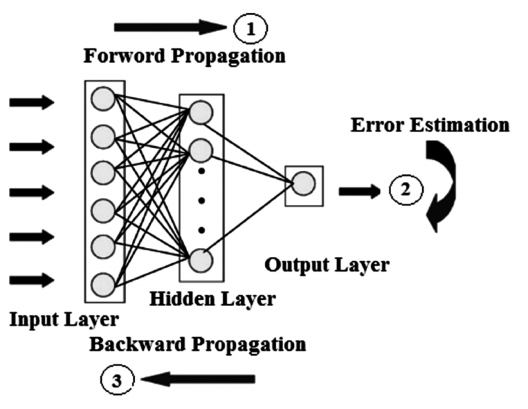
\includegraphics{img/Back-propagation-multilayer-ANN-with-one-hidden-layer.png}
\caption{ANN steps}
\end{figure}

\begin{itemize}
\tightlist
\item
  \textbf{Feed-forward} predicts output classes from the given inputs
  using the weights the network currently posseses.
\item
  \textbf{Backpropagation} calculates the error in each neuron (based on
  the predicted class and its ground truth) and updates the weights
  accordingly.
\end{itemize}

The algorithm used for the feed-forward and backpropagation is based on
the algorithm in the book
\href{https://www.cs.ubbcluj.ro/~gabis/ml/ml-books/McGrawHill\%20-\%20Machine\%20Learning\%20-Tom\%20Mitchell.pdf}{Machine
Learning (Mitchell, 1997, p.~98)}.

    We implement the \texttt{LunakArtificialNeuralNetwork} class to
represent our neural network model. The class possesses two notable
methods: - \texttt{fit(·)}: Trains a model with a given dataset, and -
\texttt{predict(·)}: Receives input data and produces predictions
according to the trained model.

The following parameters are used for \texttt{fit(·)}. 1. \texttt{X}:
\texttt{data}, training data 2. \texttt{y}: \texttt{data}, labels for
training data 3. \texttt{epochs}: \texttt{int}, the number of epochs
that will be run 4. \texttt{lr}: \texttt{float}, learning rate 5.
\texttt{momentum}: \texttt{float}, momentum (used to prevent local
minima) 6. \texttt{batch\_size}: \texttt{int}, incremental when 1
(default=\texttt{len(X)}) 7. \texttt{val\_data}:
\texttt{(X\_val,\ y\_val)}, for validation purposes
(default=\texttt{None}, will use \texttt{val\_size}=0.1) 8.
\texttt{val\_size}: \texttt{float}, used to split X and y to get
validation data (default=0)

    \begin{Verbatim}[commandchars=\\\{\}]
{\color{incolor}In [{\color{incolor}3}]:} \PY{k}{class} \PY{n+nc}{LunakArtificialNeuralNetwork}\PY{p}{:}
            \PY{k}{def} \PY{n+nf}{\PYZus{}\PYZus{}init\PYZus{}\PYZus{}}\PY{p}{(}\PY{n+nb+bp}{self}\PY{p}{,} \PY{n}{loss}\PY{o}{=}\PY{l+s+s1}{\PYZsq{}}\PY{l+s+s1}{root\PYZus{}mean\PYZus{}squared}\PY{l+s+s1}{\PYZsq{}}\PY{p}{,} \PY{n}{optimizer}\PY{o}{=}\PY{l+s+s1}{\PYZsq{}}\PY{l+s+s1}{sgd}\PY{l+s+s1}{\PYZsq{}}\PY{p}{)}\PY{p}{:}
                \PY{k}{assert} \PY{n}{loss} \PY{o}{==} \PY{l+s+s1}{\PYZsq{}}\PY{l+s+s1}{root\PYZus{}mean\PYZus{}squared}\PY{l+s+s1}{\PYZsq{}}\PY{p}{,} \PY{l+s+s1}{\PYZsq{}}\PY{l+s+s1}{loss function not supported}\PY{l+s+s1}{\PYZsq{}}
                \PY{k}{assert} \PY{n}{optimizer} \PY{o}{==} \PY{l+s+s1}{\PYZsq{}}\PY{l+s+s1}{sgd}\PY{l+s+s1}{\PYZsq{}}\PY{p}{,} \PY{l+s+s1}{\PYZsq{}}\PY{l+s+s1}{optimizer not supported}\PY{l+s+s1}{\PYZsq{}}
                \PY{n+nb+bp}{self}\PY{o}{.}\PY{n}{layers} \PY{o}{=} \PY{p}{[}\PY{p}{]}
            
            \PY{k}{def} \PY{n+nf}{add}\PY{p}{(}\PY{n+nb+bp}{self}\PY{p}{,} \PY{n}{layer}\PY{p}{)}\PY{p}{:}
                \PY{n+nb+bp}{self}\PY{o}{.}\PY{n}{layers}\PY{o}{.}\PY{n}{append}\PY{p}{(}\PY{n}{layer}\PY{p}{)}
                
            \PY{k}{def} \PY{n+nf}{feed\PYZus{}forward}\PY{p}{(}\PY{n+nb+bp}{self}\PY{p}{,} \PY{n}{X\PYZus{}instance}\PY{p}{)}\PY{p}{:}
                \PY{c+c1}{\PYZsh{} Calculate output with the first hidden layer}
                \PY{n}{output\PYZus{}list} \PY{o}{=} \PY{n+nb+bp}{self}\PY{o}{.}\PY{n}{layers}\PY{p}{[}\PY{l+m+mi}{0}\PY{p}{]}\PY{o}{.}\PY{n}{calculate\PYZus{}output}\PY{p}{(}\PY{n}{X\PYZus{}instance}\PY{p}{)}
                \PY{c+c1}{\PYZsh{} Calculate output with the second until the last layer}
                \PY{k}{for} \PY{n}{layer} \PY{o+ow}{in} \PY{n+nb+bp}{self}\PY{o}{.}\PY{n}{layers}\PY{p}{[}\PY{l+m+mi}{1}\PY{p}{:}\PY{p}{]}\PY{p}{:}
                    \PY{n}{next\PYZus{}output\PYZus{}list} \PY{o}{=} \PY{n}{layer}\PY{o}{.}\PY{n}{calculate\PYZus{}output}\PY{p}{(}\PY{n}{output\PYZus{}list}\PY{p}{)}
                    \PY{n}{output\PYZus{}list} \PY{o}{=} \PY{n}{next\PYZus{}output\PYZus{}list}
                \PY{k}{return} \PY{n}{output\PYZus{}list}\PY{o}{.}\PY{n}{copy}\PY{p}{(}\PY{p}{)}
                    
            \PY{k}{def} \PY{n+nf}{backpropagation}\PY{p}{(}\PY{n+nb+bp}{self}\PY{p}{,} \PY{n}{y\PYZus{}instance}\PY{p}{)}\PY{p}{:}
                \PY{c+c1}{\PYZsh{} Calculate local gradient for output layer}
                \PY{n}{next\PYZus{}local\PYZus{}gradient\PYZus{}list} \PY{o}{=} \PYZbs{}
                    \PY{n+nb+bp}{self}\PY{o}{.}\PY{n}{layers}\PY{p}{[}\PY{o}{\PYZhy{}}\PY{l+m+mi}{1}\PY{p}{]}\PY{o}{.}\PY{n}{calculate\PYZus{}local\PYZus{}gradient\PYZus{}output\PYZus{}layer}\PY{p}{(}\PY{p}{[}\PY{n}{y\PYZus{}instance}\PY{p}{]}\PY{p}{)}
                \PY{n}{next\PYZus{}layer\PYZus{}weight\PYZus{}matrix} \PY{o}{=} \PY{n+nb+bp}{self}\PY{o}{.}\PY{n}{layers}\PY{p}{[}\PY{o}{\PYZhy{}}\PY{l+m+mi}{1}\PY{p}{]}\PY{o}{.}\PY{n}{weight\PYZus{}matrix}
        
                \PY{c+c1}{\PYZsh{} Calculate local gradient for hidden layer(s)}
                \PY{k}{for} \PY{n}{layer\PYZus{}idx}\PY{p}{,} \PY{n}{layer} \PY{o+ow}{in} \PY{n+nb}{enumerate}\PY{p}{(}\PY{n+nb}{reversed}\PY{p}{(}\PY{n+nb+bp}{self}\PY{o}{.}\PY{n}{layers}\PY{p}{[}\PY{l+m+mi}{0}\PY{p}{:}\PY{o}{\PYZhy{}}\PY{l+m+mi}{1}\PY{p}{]}\PY{p}{)}\PY{p}{)}\PY{p}{:}
                    \PY{n}{next\PYZus{}local\PYZus{}gradient\PYZus{}list} \PY{o}{=} \PYZbs{}
                        \PY{n}{layer}\PY{o}{.}\PY{n}{calculate\PYZus{}local\PYZus{}gradient\PYZus{}hidden\PYZus{}layer}\PY{p}{(}\PY{n}{next\PYZus{}local\PYZus{}gradient\PYZus{}list}\PY{p}{,}
                                                                    \PY{n}{next\PYZus{}layer\PYZus{}weight\PYZus{}matrix}\PY{p}{)}
                    \PY{n}{next\PYZus{}layer\PYZus{}weight\PYZus{}matrix} \PY{o}{=} \PY{n}{layer}\PY{o}{.}\PY{n}{weight\PYZus{}matrix}
                    
            \PY{k}{def} \PY{n+nf}{calculate\PYZus{}delta\PYZus{}weight}\PY{p}{(}\PY{n+nb+bp}{self}\PY{p}{,} \PY{n}{X\PYZus{}instance}\PY{p}{,} \PY{n}{lr}\PY{p}{,} \PY{n}{momentum}\PY{p}{)}\PY{p}{:}
                \PY{c+c1}{\PYZsh{} Update delta weight for first hidden layer}
                \PY{n+nb+bp}{self}\PY{o}{.}\PY{n}{layers}\PY{p}{[}\PY{l+m+mi}{0}\PY{p}{]}\PY{o}{.}\PY{n}{update\PYZus{}delta\PYZus{}weight}\PY{p}{(}\PY{n}{lr}\PY{p}{,} \PY{n}{X\PYZus{}instance}\PY{p}{,} \PY{n}{momentum}\PY{p}{)}
                
                \PY{c+c1}{\PYZsh{} Update delta weight for other layers}
                \PY{k}{for} \PY{n}{layer\PYZus{}idx}\PY{p}{,} \PY{n}{layer} \PY{o+ow}{in} \PY{n+nb}{enumerate}\PY{p}{(}\PY{n+nb+bp}{self}\PY{o}{.}\PY{n}{layers}\PY{p}{[}\PY{l+m+mi}{1}\PY{p}{:}\PY{p}{]}\PY{p}{)}\PY{p}{:}
                    \PY{n}{layer}\PY{o}{.}\PY{n}{update\PYZus{}delta\PYZus{}weight}\PY{p}{(}\PY{n}{lr}\PY{p}{,} \PY{n+nb+bp}{self}\PY{o}{.}\PY{n}{layers}\PY{p}{[}\PY{n}{layer\PYZus{}idx}\PY{p}{]}\PY{o}{.}\PY{n}{output\PYZus{}list}\PY{p}{,}
                                              \PY{n}{momentum}\PY{p}{)}
            
            \PY{k}{def} \PY{n+nf}{fit}\PY{p}{(}\PY{n+nb+bp}{self}\PY{p}{,} \PY{n}{X}\PY{p}{,} \PY{n}{y}\PY{p}{,} \PY{n}{epochs}\PY{p}{,} \PY{n}{lr}\PY{p}{,} \PY{n}{momentum}\PY{o}{=}\PY{k+kc}{None}\PY{p}{,}
                    \PY{n}{batch\PYZus{}size}\PY{o}{=}\PY{k+kc}{None}\PY{p}{,} \PY{n}{val\PYZus{}data}\PY{o}{=}\PY{k+kc}{None}\PY{p}{,} \PY{n}{val\PYZus{}size}\PY{o}{=}\PY{l+m+mi}{0}\PY{p}{)}\PY{p}{:}
                \PY{k}{assert} \PY{n}{X}\PY{o}{.}\PY{n}{shape}\PY{p}{[}\PY{l+m+mi}{1}\PY{p}{]} \PY{o}{==} \PY{n+nb+bp}{self}\PY{o}{.}\PY{n}{layers}\PY{p}{[}\PY{l+m+mi}{0}\PY{p}{]}\PY{o}{.}\PY{n}{input\PYZus{}dim}\PY{p}{,} \PYZbs{}
                    \PY{l+s+s1}{\PYZsq{}}\PY{l+s+s1}{Input dimension must be same with the column}\PY{l+s+s1}{\PYZsq{}}
                \PY{n+nb+bp}{self}\PY{o}{.}\PY{n}{classes\PYZus{}} \PY{o}{=} \PY{n}{np}\PY{o}{.}\PY{n}{unique}\PY{p}{(}\PY{n}{y}\PY{p}{)}
                
                \PY{k}{if} \PY{n}{batch\PYZus{}size} \PY{o}{==} \PY{k+kc}{None}\PY{p}{:}
                    \PY{n}{batch\PYZus{}size} \PY{o}{=} \PY{n+nb}{len}\PY{p}{(}\PY{n}{X}\PY{p}{)}
                    
                \PY{k}{if} \PY{n}{val\PYZus{}data} \PY{o+ow}{is} \PY{k+kc}{None}\PY{p}{:}
                    \PY{n}{val\PYZus{}size} \PY{o}{=} \PY{l+m+mf}{0.1}
                    \PY{n}{X}\PY{p}{,} \PY{n}{X\PYZus{}val}\PY{p}{,} \PY{n}{y}\PY{p}{,} \PY{n}{y\PYZus{}val} \PY{o}{=} \PY{n}{train\PYZus{}test\PYZus{}split}\PY{p}{(}\PY{n}{X}\PY{p}{,} \PY{n}{y}\PY{p}{,} \PY{n}{test\PYZus{}size}\PY{o}{=}\PY{n}{val\PYZus{}size}\PY{p}{)}
                \PY{k}{else}\PY{p}{:}
                    \PY{n}{X\PYZus{}val} \PY{o}{=} \PY{n}{val\PYZus{}data}\PY{p}{[}\PY{l+m+mi}{0}\PY{p}{]}
                    \PY{n}{y\PYZus{}val} \PY{o}{=} \PY{n}{val\PYZus{}data}\PY{p}{[}\PY{l+m+mi}{1}\PY{p}{]}
                    
                \PY{n+nb}{print}\PY{p}{(}\PY{l+s+s1}{\PYZsq{}}\PY{l+s+s1}{Train on }\PY{l+s+si}{\PYZob{}\PYZcb{}}\PY{l+s+s1}{ samples, validate on }\PY{l+s+si}{\PYZob{}\PYZcb{}}\PY{l+s+s1}{ samples}\PY{l+s+s1}{\PYZsq{}}\PY{o}{.}\PY{n}{format}\PY{p}{(}\PY{n+nb}{len}\PY{p}{(}\PY{n}{X}\PY{p}{)}\PY{p}{,}
                                                                           \PY{n+nb}{len}\PY{p}{(}\PY{n}{X\PYZus{}val}\PY{p}{)}\PY{p}{)}\PY{p}{)}
                
                \PY{k}{if} \PY{n}{val\PYZus{}data} \PY{o+ow}{is} \PY{o+ow}{not} \PY{k+kc}{None} \PY{o+ow}{and} \PY{n}{val\PYZus{}size} \PY{o}{!=} \PY{l+m+mi}{0}\PY{p}{:}
                    \PY{n+nb}{print}\PY{p}{(}\PY{l+s+s1}{\PYZsq{}}\PY{l+s+s1}{Validation data will be used instead of val\PYZus{}size.}\PY{l+s+s1}{\PYZsq{}}\PY{p}{)}
                    
                \PY{k}{for} \PY{n}{epoch} \PY{o+ow}{in} \PY{n+nb}{range}\PY{p}{(}\PY{n}{epochs}\PY{p}{)}\PY{p}{:}
                    \PY{n}{delta} \PY{o}{=} \PY{n}{batch\PYZus{}size}
                    
                    \PY{k}{with} \PY{n}{tnrange}\PY{p}{(}\PY{l+m+mi}{0}\PY{p}{,} \PY{n+nb}{len}\PY{p}{(}\PY{n}{X}\PY{p}{)}\PY{p}{,} \PY{n}{delta}\PY{p}{,}
                                 \PY{n}{desc}\PY{o}{=}\PY{l+s+s1}{\PYZsq{}}\PY{l+s+s1}{Epoch }\PY{l+s+si}{\PYZob{}\PYZcb{}}\PY{l+s+s1}{\PYZsq{}}\PY{o}{.}\PY{n}{format}\PY{p}{(}\PY{n}{epoch} \PY{o}{+} \PY{l+m+mi}{1}\PY{p}{)}\PY{p}{)} \PY{k}{as} \PY{n}{pbar}\PY{p}{:}
                        \PY{k}{for} \PY{n}{start} \PY{o+ow}{in} \PY{n}{pbar}\PY{p}{:}
                            \PY{n}{X\PYZus{}batch} \PY{o}{=} \PY{n}{X}\PY{p}{[}\PY{n}{start}\PY{p}{:}\PY{n}{start}\PY{o}{+}\PY{n}{delta}\PY{p}{]}
                            \PY{n}{y\PYZus{}batch} \PY{o}{=} \PY{n}{y}\PY{p}{[}\PY{n}{start}\PY{p}{:}\PY{n}{start}\PY{o}{+}\PY{n}{delta}\PY{p}{]}
        
                            \PY{k}{for} \PY{n}{idx}\PY{p}{,} \PY{n}{X\PYZus{}instance} \PY{o+ow}{in} \PY{n+nb}{enumerate}\PY{p}{(}\PY{n}{X\PYZus{}batch}\PY{p}{)}\PY{p}{:}
                                \PY{n+nb+bp}{self}\PY{o}{.}\PY{n}{feed\PYZus{}forward}\PY{p}{(}\PY{n}{X\PYZus{}instance}\PY{p}{)}
                                \PY{n+nb+bp}{self}\PY{o}{.}\PY{n}{backpropagation}\PY{p}{(}\PY{n}{y\PYZus{}batch}\PY{p}{[}\PY{n}{idx}\PY{p}{]}\PY{p}{[}\PY{l+m+mi}{0}\PY{p}{]}\PY{p}{)}
                                \PY{n+nb+bp}{self}\PY{o}{.}\PY{n}{calculate\PYZus{}delta\PYZus{}weight}\PY{p}{(}\PY{n}{X\PYZus{}instance}\PY{p}{,} \PY{n}{lr}\PY{p}{,} \PY{n}{momentum}\PY{p}{)}
        
                            \PY{k}{for} \PY{n}{layer} \PY{o+ow}{in} \PY{n+nb+bp}{self}\PY{o}{.}\PY{n}{layers}\PY{p}{:}
                                \PY{n}{layer}\PY{o}{.}\PY{n}{update\PYZus{}weight}\PY{p}{(}\PY{p}{)}
                                \PY{n}{layer}\PY{o}{.}\PY{n}{init\PYZus{}delta\PYZus{}weight\PYZus{}zero}\PY{p}{(}\PY{p}{)}
        
                            \PY{n}{pred} \PY{o}{=} \PY{n+nb+bp}{self}\PY{o}{.}\PY{n}{predict}\PY{p}{(}\PY{n}{X}\PY{p}{)}
                            \PY{n}{pred\PYZus{}val} \PY{o}{=} \PY{n+nb+bp}{self}\PY{o}{.}\PY{n}{predict}\PY{p}{(}\PY{n}{X\PYZus{}val}\PY{p}{)}
                            
                            \PY{n}{pred\PYZus{}proba} \PY{o}{=} \PY{n+nb+bp}{self}\PY{o}{.}\PY{n}{predict\PYZus{}proba}\PY{p}{(}\PY{n}{X}\PY{p}{)}
                            \PY{n}{pred\PYZus{}proba\PYZus{}val} \PY{o}{=} \PY{n+nb+bp}{self}\PY{o}{.}\PY{n}{predict\PYZus{}proba}\PY{p}{(}\PY{n}{X\PYZus{}val}\PY{p}{)}
        
                            \PY{n}{acc} \PY{o}{=} \PY{n+nb+bp}{self}\PY{o}{.}\PY{n}{calculate\PYZus{}accuracy}\PY{p}{(}\PY{n}{y}\PY{p}{,} \PY{n}{pred}\PY{p}{)}
                            \PY{n}{val\PYZus{}acc} \PY{o}{=} \PY{n+nb+bp}{self}\PY{o}{.}\PY{n}{calculate\PYZus{}accuracy}\PY{p}{(}\PY{n}{y\PYZus{}val}\PY{p}{,} \PY{n}{pred\PYZus{}val}\PY{p}{)}
                            \PY{n}{loss} \PY{o}{=} \PY{n}{mean\PYZus{}squared\PYZus{}error}\PY{p}{(}\PY{n}{y}\PY{p}{,} \PY{n}{pred\PYZus{}proba}\PY{p}{)}
                            \PY{n}{val\PYZus{}loss} \PY{o}{=} \PY{n}{mean\PYZus{}squared\PYZus{}error}\PY{p}{(}\PY{n}{y\PYZus{}val}\PY{p}{,} \PY{n}{pred\PYZus{}proba\PYZus{}val}\PY{p}{)}
        
                            \PY{n}{postfix} \PY{o}{=} \PY{p}{\PYZob{}}
                                \PY{l+s+s1}{\PYZsq{}}\PY{l+s+s1}{loss}\PY{l+s+s1}{\PYZsq{}}\PY{p}{:} \PY{n}{loss}\PY{p}{,}
                                \PY{l+s+s1}{\PYZsq{}}\PY{l+s+s1}{acc}\PY{l+s+s1}{\PYZsq{}}\PY{p}{:} \PY{n}{acc}\PY{p}{,}
                                \PY{l+s+s1}{\PYZsq{}}\PY{l+s+s1}{val\PYZus{}loss}\PY{l+s+s1}{\PYZsq{}}\PY{p}{:} \PY{n}{val\PYZus{}loss}\PY{p}{,}
                                \PY{l+s+s1}{\PYZsq{}}\PY{l+s+s1}{val\PYZus{}acc}\PY{l+s+s1}{\PYZsq{}}\PY{p}{:} \PY{n}{val\PYZus{}acc}
                            \PY{p}{\PYZcb{}}
                            \PY{n}{pbar}\PY{o}{.}\PY{n}{set\PYZus{}postfix}\PY{p}{(}\PY{n}{postfix}\PY{p}{,} \PY{n}{refresh}\PY{o}{=}\PY{k+kc}{True}\PY{p}{)}
            
            \PY{k}{def} \PY{n+nf}{predict\PYZus{}proba}\PY{p}{(}\PY{n+nb+bp}{self}\PY{p}{,} \PY{n}{X}\PY{p}{)}\PY{p}{:}
                \PY{n}{predictions} \PY{o}{=} \PY{p}{[}\PY{p}{]}
                \PY{k}{for} \PY{n}{idx}\PY{p}{,} \PY{n}{X\PYZus{}instance} \PY{o+ow}{in} \PY{n+nb}{enumerate}\PY{p}{(}\PY{n}{X}\PY{p}{)}\PY{p}{:}
                    \PY{n}{X\PYZus{}pred} \PY{o}{=} \PY{n+nb+bp}{self}\PY{o}{.}\PY{n}{feed\PYZus{}forward}\PY{p}{(}\PY{n}{X\PYZus{}instance}\PY{p}{)}
                    \PY{n}{predictions}\PY{o}{.}\PY{n}{append}\PY{p}{(}\PY{p}{[}\PY{n}{np}\PY{o}{.}\PY{n}{mean}\PY{p}{(}\PY{n}{X\PYZus{}pred}\PY{o}{.}\PY{n}{copy}\PY{p}{(}\PY{p}{)}\PY{p}{)}\PY{p}{]}\PY{p}{)}
                \PY{k}{return} \PY{n}{predictions}
            
            \PY{k}{def} \PY{n+nf}{predict}\PY{p}{(}\PY{n+nb+bp}{self}\PY{p}{,} \PY{n}{X}\PY{p}{)}\PY{p}{:}
                \PY{n}{predictions} \PY{o}{=} \PY{p}{[}\PY{p}{]}
                \PY{k}{for} \PY{n}{idx}\PY{p}{,} \PY{n}{X\PYZus{}instance} \PY{o+ow}{in} \PY{n+nb}{enumerate}\PY{p}{(}\PY{n}{X}\PY{p}{)}\PY{p}{:}
                    \PY{n}{X\PYZus{}pred\PYZus{}proba} \PY{o}{=} \PY{n+nb+bp}{self}\PY{o}{.}\PY{n}{feed\PYZus{}forward}\PY{p}{(}\PY{n}{X\PYZus{}instance}\PY{p}{)}
                    \PY{n}{X\PYZus{}pred} \PY{o}{=} \PY{n+nb}{min}\PY{p}{(}\PY{n+nb+bp}{self}\PY{o}{.}\PY{n}{classes\PYZus{}}\PY{p}{,}
                                 \PY{n}{key}\PY{o}{=}\PY{k}{lambda} \PY{n}{pred\PYZus{}class}\PY{p}{:}\PY{n+nb}{abs}\PY{p}{(}\PY{n}{pred\PYZus{}class} \PY{o}{\PYZhy{}} \PY{n}{np}\PY{o}{.}\PY{n}{mean}\PY{p}{(}\PY{n}{X\PYZus{}pred\PYZus{}proba}\PY{p}{)}\PY{p}{)}\PY{p}{)}
                    \PY{n}{predictions}\PY{o}{.}\PY{n}{append}\PY{p}{(}\PY{p}{[}\PY{n}{X\PYZus{}pred}\PY{p}{]}\PY{p}{)}
                \PY{k}{return} \PY{n}{predictions}
            
            \PY{k}{def} \PY{n+nf}{calculate\PYZus{}accuracy}\PY{p}{(}\PY{n+nb+bp}{self}\PY{p}{,} \PY{n}{y\PYZus{}true}\PY{p}{,} \PY{n}{y\PYZus{}pred}\PY{p}{)}\PY{p}{:}
                \PY{k}{if} \PY{n+nb}{len}\PY{p}{(}\PY{n}{confusion\PYZus{}matrix}\PY{p}{(}\PY{n}{y\PYZus{}true}\PY{p}{,} \PY{n}{y\PYZus{}pred}\PY{p}{)}\PY{o}{.}\PY{n}{ravel}\PY{p}{(}\PY{p}{)}\PY{p}{)} \PY{o}{\PYZgt{}} \PY{l+m+mi}{1}\PY{p}{:}
                    \PY{n}{tn}\PY{p}{,} \PY{n}{fp}\PY{p}{,} \PY{n}{fn}\PY{p}{,} \PY{n}{tp} \PY{o}{=} \PY{n}{confusion\PYZus{}matrix}\PY{p}{(}\PY{n}{y\PYZus{}true}\PY{p}{,} \PY{n}{y\PYZus{}pred}\PY{p}{)}\PY{o}{.}\PY{n}{ravel}\PY{p}{(}\PY{p}{)}
                \PY{k}{else}\PY{p}{:}
                    \PY{n}{tp} \PY{o}{=} \PY{n}{confusion\PYZus{}matrix}\PY{p}{(}\PY{n}{y\PYZus{}true}\PY{p}{,} \PY{n}{y\PYZus{}pred}\PY{p}{)}\PY{o}{.}\PY{n}{ravel}\PY{p}{(}\PY{p}{)}\PY{p}{[}\PY{l+m+mi}{0}\PY{p}{]}
                    \PY{n}{fp} \PY{o}{=} \PY{l+m+mi}{0}
                    \PY{n}{fn} \PY{o}{=} \PY{l+m+mi}{0}
                    \PY{n}{tn} \PY{o}{=} \PY{l+m+mi}{0}
                \PY{k}{return} \PY{p}{(}\PY{n}{tp} \PY{o}{+} \PY{n}{tn}\PY{p}{)} \PY{o}{/} \PY{p}{(}\PY{n}{tp} \PY{o}{+} \PY{n}{tn} \PY{o}{+} \PY{n}{fp} \PY{o}{+} \PY{n}{fn}\PY{p}{)}
\end{Verbatim}


    \hypertarget{testing-our-implementation}{%
\section{Testing our implementation}\label{testing-our-implementation}}

    To test whether Lunak works correctly, we train both our model and a
Keras ANN model as baseline, then compare their results and performance.

    \begin{Verbatim}[commandchars=\\\{\}]
{\color{incolor}In [{\color{incolor}4}]:} \PY{k+kn}{from} \PY{n+nn}{scipy}\PY{n+nn}{.}\PY{n+nn}{io}\PY{n+nn}{.}\PY{n+nn}{arff} \PY{k}{import} \PY{n}{loadarff}
        \PY{k+kn}{import} \PY{n+nn}{pandas} \PY{k}{as} \PY{n+nn}{pd}
        \PY{k+kn}{from} \PY{n+nn}{IPython}\PY{n+nn}{.}\PY{n+nn}{utils} \PY{k}{import} \PY{n}{io}
\end{Verbatim}


    Our dataset is the Play Tennis dataset, obtained from the
\href{http://storm.cis.fordham.edu/~gweiss/data-mining/weka-data/weather.arff}{Weka
Data Sets}.

    \begin{Verbatim}[commandchars=\\\{\}]
{\color{incolor}In [{\color{incolor}5}]:} \PY{n}{raw\PYZus{}data} \PY{o}{=} \PY{n}{loadarff}\PY{p}{(}\PY{l+s+s1}{\PYZsq{}}\PY{l+s+s1}{dataset/weather.arff}\PY{l+s+s1}{\PYZsq{}}\PY{p}{)}
        \PY{n}{data} \PY{o}{=} \PY{n}{pd}\PY{o}{.}\PY{n}{DataFrame}\PY{p}{(}\PY{n}{raw\PYZus{}data}\PY{p}{[}\PY{l+m+mi}{0}\PY{p}{]}\PY{p}{)}
        \PY{n}{data}\PY{o}{.}\PY{n}{head}\PY{p}{(}\PY{p}{)}
\end{Verbatim}


\begin{Verbatim}[commandchars=\\\{\}]
{\color{outcolor}Out[{\color{outcolor}5}]:}        outlook  temperature  humidity     windy    play
        0     b'sunny'         85.0      85.0  b'FALSE'   b'no'
        1     b'sunny'         80.0      90.0   b'TRUE'   b'no'
        2  b'overcast'         83.0      86.0  b'FALSE'  b'yes'
        3     b'rainy'         70.0      96.0  b'FALSE'  b'yes'
        4     b'rainy'         68.0      80.0  b'FALSE'  b'yes'
\end{Verbatim}
            
    \hypertarget{preprocessing}{%
\subsection{Preprocessing}\label{preprocessing}}

    Before we train our model, we must first preprocess our data, as the
data types of our chosen dataset cannot be fed to our ANN
out-of-the-box.

    \begin{Verbatim}[commandchars=\\\{\}]
{\color{incolor}In [{\color{incolor}6}]:} \PY{k}{def} \PY{n+nf}{convert\PYZus{}to\PYZus{}binary\PYZus{}vector}\PY{p}{(}\PY{n}{data}\PY{p}{)}\PY{p}{:}
            \PY{k}{return} \PY{n}{pd}\PY{o}{.}\PY{n}{get\PYZus{}dummies}\PY{p}{(}\PY{n}{data}\PY{p}{)}
\end{Verbatim}


    First, we decode strings and boolean data in the dataset as UTF-8.

    \begin{Verbatim}[commandchars=\\\{\}]
{\color{incolor}In [{\color{incolor}7}]:} \PY{k}{for} \PY{n}{idx}\PY{p}{,} \PY{n}{column} \PY{o+ow}{in} \PY{n+nb}{enumerate}\PY{p}{(}\PY{p}{[}\PY{l+s+s1}{\PYZsq{}}\PY{l+s+s1}{outlook}\PY{l+s+s1}{\PYZsq{}}\PY{p}{,} \PY{l+s+s1}{\PYZsq{}}\PY{l+s+s1}{windy}\PY{l+s+s1}{\PYZsq{}}\PY{p}{,} \PY{l+s+s1}{\PYZsq{}}\PY{l+s+s1}{play}\PY{l+s+s1}{\PYZsq{}}\PY{p}{]}\PY{p}{)}\PY{p}{:}
            \PY{n}{data}\PY{p}{[}\PY{n}{column}\PY{p}{]} \PY{o}{=} \PY{n}{data}\PY{p}{[}\PY{n}{column}\PY{p}{]}\PY{o}{.}\PY{n}{str}\PY{o}{.}\PY{n}{decode}\PY{p}{(}\PY{l+s+s1}{\PYZsq{}}\PY{l+s+s1}{utf\PYZhy{}8}\PY{l+s+s1}{\PYZsq{}}\PY{p}{)}
\end{Verbatim}


    Then, string categoricals in the data (i.e., \texttt{outlook} and
\texttt{windy}) are converted to one-hot vectors.

    \begin{Verbatim}[commandchars=\\\{\}]
{\color{incolor}In [{\color{incolor}8}]:} \PY{n}{bv\PYZus{}outlook} \PY{o}{=} \PY{n}{convert\PYZus{}to\PYZus{}binary\PYZus{}vector}\PY{p}{(}\PY{n}{data}\PY{p}{[}\PY{l+s+s1}{\PYZsq{}}\PY{l+s+s1}{outlook}\PY{l+s+s1}{\PYZsq{}}\PY{p}{]}\PY{p}{)}
        \PY{n}{bv\PYZus{}outlook}\PY{o}{.}\PY{n}{head}\PY{p}{(}\PY{p}{)}
\end{Verbatim}


\begin{Verbatim}[commandchars=\\\{\}]
{\color{outcolor}Out[{\color{outcolor}8}]:}    overcast  rainy  sunny
        0         0      0      1
        1         0      0      1
        2         1      0      0
        3         0      1      0
        4         0      1      0
\end{Verbatim}
            
    \begin{Verbatim}[commandchars=\\\{\}]
{\color{incolor}In [{\color{incolor}9}]:} \PY{n}{bv\PYZus{}windy} \PY{o}{=} \PY{n}{convert\PYZus{}to\PYZus{}binary\PYZus{}vector}\PY{p}{(}\PY{n}{data}\PY{p}{[}\PY{l+s+s1}{\PYZsq{}}\PY{l+s+s1}{windy}\PY{l+s+s1}{\PYZsq{}}\PY{p}{]}\PY{p}{)}
        \PY{n}{bv\PYZus{}windy}\PY{o}{.}\PY{n}{head}\PY{p}{(}\PY{p}{)}
\end{Verbatim}


\begin{Verbatim}[commandchars=\\\{\}]
{\color{outcolor}Out[{\color{outcolor}9}]:}    FALSE  TRUE
        0      1     0
        1      0     1
        2      1     0
        3      1     0
        4      1     0
\end{Verbatim}
            
    We drop the categorical \texttt{outlook} and \texttt{windy} data and
concatenate our one-hot vectors to the dataset.

    \begin{Verbatim}[commandchars=\\\{\}]
{\color{incolor}In [{\color{incolor}10}]:} \PY{n}{preproc\PYZus{}data} \PY{o}{=} \PY{n}{data}\PY{o}{.}\PY{n}{drop}\PY{p}{(}\PY{l+s+s1}{\PYZsq{}}\PY{l+s+s1}{outlook}\PY{l+s+s1}{\PYZsq{}}\PY{p}{,} \PY{l+m+mi}{1}\PY{p}{)}\PY{o}{.}\PY{n}{drop}\PY{p}{(}\PY{l+s+s1}{\PYZsq{}}\PY{l+s+s1}{windy}\PY{l+s+s1}{\PYZsq{}}\PY{p}{,} \PY{l+m+mi}{1}\PY{p}{)}
         \PY{n}{preprocessed\PYZus{}data} \PY{o}{=} \PY{n}{pd}\PY{o}{.}\PY{n}{concat}\PY{p}{(}\PY{p}{[}\PY{n}{bv\PYZus{}outlook}\PY{p}{,} \PY{n}{bv\PYZus{}windy}\PY{p}{,} \PY{n}{preproc\PYZus{}data}\PY{p}{]}\PY{p}{,} \PY{n}{axis}\PY{o}{=}\PY{l+m+mi}{1}\PY{p}{)}
\end{Verbatim}


    Our target column, \texttt{play}, is processed as categorical data.

    \begin{Verbatim}[commandchars=\\\{\}]
{\color{incolor}In [{\color{incolor}11}]:} \PY{n}{preproc\PYZus{}data}\PY{p}{[}\PY{l+s+s1}{\PYZsq{}}\PY{l+s+s1}{play}\PY{l+s+s1}{\PYZsq{}}\PY{p}{]} \PY{o}{=} \PY{n}{preproc\PYZus{}data}\PY{p}{[}\PY{l+s+s1}{\PYZsq{}}\PY{l+s+s1}{play}\PY{l+s+s1}{\PYZsq{}}\PY{p}{]}\PY{o}{.}\PY{n}{astype}\PY{p}{(}\PY{l+s+s1}{\PYZsq{}}\PY{l+s+s1}{category}\PY{l+s+s1}{\PYZsq{}}\PY{p}{)}
         \PY{n}{preprocessed\PYZus{}data}\PY{o}{.}\PY{n}{head}\PY{p}{(}\PY{p}{)}
\end{Verbatim}


\begin{Verbatim}[commandchars=\\\{\}]
{\color{outcolor}Out[{\color{outcolor}11}]:}    overcast  rainy  sunny  FALSE  TRUE  temperature  humidity play
         0         0      0      1      1     0         85.0      85.0   no
         1         0      0      1      0     1         80.0      90.0   no
         2         1      0      0      1     0         83.0      86.0  yes
         3         0      1      0      1     0         70.0      96.0  yes
         4         0      1      0      1     0         68.0      80.0  yes
\end{Verbatim}
            
    The, the \texttt{play} column is converted to binary 0/1 integers.

    \begin{Verbatim}[commandchars=\\\{\}]
{\color{incolor}In [{\color{incolor}12}]:} \PY{n}{y} \PY{o}{=} \PY{n}{pd}\PY{o}{.}\PY{n}{DataFrame}\PY{p}{(}\PY{p}{\PYZob{}}\PY{l+s+s1}{\PYZsq{}}\PY{l+s+s1}{play}\PY{l+s+s1}{\PYZsq{}}\PY{p}{:} \PY{n}{preproc\PYZus{}data}\PY{p}{[}\PY{l+s+s1}{\PYZsq{}}\PY{l+s+s1}{play}\PY{l+s+s1}{\PYZsq{}}\PY{p}{]}\PY{o}{.}\PY{n}{cat}\PY{o}{.}\PY{n}{codes}\PY{p}{\PYZcb{}}\PY{p}{)}
         \PY{n}{y}\PY{o}{.}\PY{n}{head}\PY{p}{(}\PY{p}{)}
\end{Verbatim}


\begin{Verbatim}[commandchars=\\\{\}]
{\color{outcolor}Out[{\color{outcolor}12}]:}    play
         0     0
         1     0
         2     1
         3     1
         4     1
\end{Verbatim}
            
    For training, we delete our target column from the dataset.

    \begin{Verbatim}[commandchars=\\\{\}]
{\color{incolor}In [{\color{incolor}13}]:} \PY{n}{X} \PY{o}{=} \PY{n}{preprocessed\PYZus{}data}\PY{o}{.}\PY{n}{drop}\PY{p}{(}\PY{l+s+s1}{\PYZsq{}}\PY{l+s+s1}{play}\PY{l+s+s1}{\PYZsq{}}\PY{p}{,} \PY{l+m+mi}{1}\PY{p}{)}
\end{Verbatim}


    We then cast all data remaining in the dataset as floats.

    \begin{Verbatim}[commandchars=\\\{\}]
{\color{incolor}In [{\color{incolor}14}]:} \PY{k}{for} \PY{n}{column} \PY{o+ow}{in} \PY{n}{X}\PY{o}{.}\PY{n}{columns}\PY{p}{:}
             \PY{n}{X}\PY{p}{[}\PY{n}{column}\PY{p}{]} \PY{o}{=} \PY{n}{X}\PY{p}{[}\PY{n}{column}\PY{p}{]}\PY{o}{.}\PY{n}{astype}\PY{p}{(}\PY{l+s+s1}{\PYZsq{}}\PY{l+s+s1}{float}\PY{l+s+s1}{\PYZsq{}}\PY{p}{)}
\end{Verbatim}


    We normalize real number data (\texttt{temperature} and
\texttt{humidity}) to \([0, 1]\).

    \begin{Verbatim}[commandchars=\\\{\}]
{\color{incolor}In [{\color{incolor}15}]:} \PY{k}{for} \PY{n}{column} \PY{o+ow}{in} \PY{p}{[}\PY{l+s+s1}{\PYZsq{}}\PY{l+s+s1}{temperature}\PY{l+s+s1}{\PYZsq{}}\PY{p}{,} \PY{l+s+s1}{\PYZsq{}}\PY{l+s+s1}{humidity}\PY{l+s+s1}{\PYZsq{}}\PY{p}{]}\PY{p}{:}
             \PY{n}{X}\PY{p}{[}\PY{n}{column}\PY{p}{]} \PY{o}{=} \PY{p}{(}\PY{n}{X}\PY{p}{[}\PY{n}{column}\PY{p}{]} \PY{o}{\PYZhy{}} \PY{n+nb}{min}\PY{p}{(}\PY{n}{X}\PY{p}{[}\PY{n}{column}\PY{p}{]}\PY{p}{)}\PY{p}{)} \PY{o}{/} \PY{p}{(}\PY{n+nb}{max}\PY{p}{(}\PY{n}{X}\PY{p}{[}\PY{n}{column}\PY{p}{]}\PY{p}{)} \PY{o}{\PYZhy{}} \PY{n+nb}{min}\PY{p}{(}\PY{n}{X}\PY{p}{[}\PY{n}{column}\PY{p}{]}\PY{p}{)}\PY{p}{)}
\end{Verbatim}


    \begin{Verbatim}[commandchars=\\\{\}]
{\color{incolor}In [{\color{incolor}16}]:} \PY{n}{X}\PY{o}{.}\PY{n}{head}\PY{p}{(}\PY{p}{)}
\end{Verbatim}


\begin{Verbatim}[commandchars=\\\{\}]
{\color{outcolor}Out[{\color{outcolor}16}]:}    overcast  rainy  sunny  FALSE  TRUE  temperature  humidity
         0       0.0    0.0    1.0    1.0   0.0     1.000000  0.645161
         1       0.0    0.0    1.0    0.0   1.0     0.761905  0.806452
         2       1.0    0.0    0.0    1.0   0.0     0.904762  0.677419
         3       0.0    1.0    0.0    1.0   0.0     0.285714  1.000000
         4       0.0    1.0    0.0    1.0   0.0     0.190476  0.483871
\end{Verbatim}
            
    We also cast our target labels to float.

    \begin{Verbatim}[commandchars=\\\{\}]
{\color{incolor}In [{\color{incolor}17}]:} \PY{n}{y} \PY{o}{=} \PY{n}{y}\PY{o}{.}\PY{n}{astype}\PY{p}{(}\PY{l+s+s1}{\PYZsq{}}\PY{l+s+s1}{float}\PY{l+s+s1}{\PYZsq{}}\PY{p}{)}
\end{Verbatim}


    Both our dataset and our target labels are converted to \texttt{numpy}
arrays for faster processing.

    \begin{Verbatim}[commandchars=\\\{\}]
{\color{incolor}In [{\color{incolor}18}]:} \PY{n}{X} \PY{o}{=} \PY{n}{np}\PY{o}{.}\PY{n}{array}\PY{p}{(}\PY{n}{X}\PY{p}{)}
         \PY{n}{y} \PY{o}{=} \PY{n}{np}\PY{o}{.}\PY{n}{array}\PY{p}{(}\PY{n}{y}\PY{p}{)}
\end{Verbatim}


    The following is our preprocessed data and their labels. We shall feed
this preprocessed data into our ANN implementations.

    \begin{Verbatim}[commandchars=\\\{\}]
{\color{incolor}In [{\color{incolor}19}]:} \PY{n}{X}
\end{Verbatim}


\begin{Verbatim}[commandchars=\\\{\}]
{\color{outcolor}Out[{\color{outcolor}19}]:} array([[0.        , 0.        , 1.        , 1.        , 0.        ,
                 1.        , 0.64516129],
                [0.        , 0.        , 1.        , 0.        , 1.        ,
                 0.76190476, 0.80645161],
                [1.        , 0.        , 0.        , 1.        , 0.        ,
                 0.9047619 , 0.67741935],
                [0.        , 1.        , 0.        , 1.        , 0.        ,
                 0.28571429, 1.        ],
                [0.        , 1.        , 0.        , 1.        , 0.        ,
                 0.19047619, 0.48387097],
                [0.        , 1.        , 0.        , 0.        , 1.        ,
                 0.04761905, 0.16129032],
                [1.        , 0.        , 0.        , 0.        , 1.        ,
                 0.        , 0.        ],
                [0.        , 0.        , 1.        , 1.        , 0.        ,
                 0.38095238, 0.96774194],
                [0.        , 0.        , 1.        , 1.        , 0.        ,
                 0.23809524, 0.16129032],
                [0.        , 1.        , 0.        , 1.        , 0.        ,
                 0.52380952, 0.48387097],
                [0.        , 0.        , 1.        , 0.        , 1.        ,
                 0.52380952, 0.16129032],
                [1.        , 0.        , 0.        , 0.        , 1.        ,
                 0.38095238, 0.80645161],
                [1.        , 0.        , 0.        , 1.        , 0.        ,
                 0.80952381, 0.32258065],
                [0.        , 1.        , 0.        , 0.        , 1.        ,
                 0.33333333, 0.83870968]])
\end{Verbatim}
            
    \begin{Verbatim}[commandchars=\\\{\}]
{\color{incolor}In [{\color{incolor}20}]:} \PY{n}{y}
\end{Verbatim}


\begin{Verbatim}[commandchars=\\\{\}]
{\color{outcolor}Out[{\color{outcolor}20}]:} array([[0.],
                [0.],
                [1.],
                [1.],
                [1.],
                [0.],
                [1.],
                [0.],
                [1.],
                [1.],
                [1.],
                [1.],
                [1.],
                [0.]])
\end{Verbatim}
            
    \hypertarget{hold-out-split}{%
\subsubsection{Hold-out split}\label{hold-out-split}}

    For training and validation, we employ a 90-10 holdout validation
scheme, i.e., 90\% data is used for training, while the remaining 10\%
is used for validation.

    \begin{Verbatim}[commandchars=\\\{\}]
{\color{incolor}In [{\color{incolor}21}]:} \PY{k+kn}{from} \PY{n+nn}{sklearn}\PY{n+nn}{.}\PY{n+nn}{model\PYZus{}selection} \PY{k}{import} \PY{n}{train\PYZus{}test\PYZus{}split}
\end{Verbatim}


    \begin{Verbatim}[commandchars=\\\{\}]
{\color{incolor}In [{\color{incolor}22}]:} \PY{n}{X}\PY{p}{,} \PY{n}{X\PYZus{}val}\PY{p}{,} \PY{n}{y}\PY{p}{,} \PY{n}{y\PYZus{}val} \PY{o}{=} \PY{n}{train\PYZus{}test\PYZus{}split}\PY{p}{(}\PY{n}{X}\PY{p}{,} \PY{n}{y}\PY{p}{,} \PY{n}{test\PYZus{}size}\PY{o}{=}\PY{l+m+mf}{0.1}\PY{p}{)}
\end{Verbatim}


    \hypertarget{building-and-training-our-models}{%
\subsection{Building and training our
models}\label{building-and-training-our-models}}

We shall now build, train, and test Lunak and Keras.

    \hypertarget{lunak}{%
\subsubsection{Lunak}\label{lunak}}

    We shall first initialize our Lunak ANN model.

    \begin{Verbatim}[commandchars=\\\{\}]
{\color{incolor}In [{\color{incolor}23}]:} \PY{n}{lunak\PYZus{}ann} \PY{o}{=} \PY{n}{LunakArtificialNeuralNetwork}\PY{p}{(}\PY{p}{)}
\end{Verbatim}


    On our model, we add a hidden layer with two units and an output layer
with one unit.

    \begin{Verbatim}[commandchars=\\\{\}]
{\color{incolor}In [{\color{incolor}24}]:} \PY{n}{lunak\PYZus{}ann}\PY{o}{.}\PY{n}{add}\PY{p}{(}\PY{n}{LunakDense}\PY{p}{(}\PY{l+m+mi}{2}\PY{p}{,} \PY{l+s+s1}{\PYZsq{}}\PY{l+s+s1}{sigmoid}\PY{l+s+s1}{\PYZsq{}}\PY{p}{,} \PY{l+m+mi}{7}\PY{p}{,} \PY{l+s+s1}{\PYZsq{}}\PY{l+s+s1}{uniform}\PY{l+s+s1}{\PYZsq{}}\PY{p}{,} \PY{n}{use\PYZus{}bias}\PY{o}{=}\PY{k+kc}{True}\PY{p}{,} \PY{n}{seed}\PY{o}{=}\PY{l+m+mi}{5}\PY{p}{)}\PY{p}{)}
         \PY{n}{lunak\PYZus{}ann}\PY{o}{.}\PY{n}{add}\PY{p}{(}\PY{n}{LunakDense}\PY{p}{(}\PY{l+m+mi}{1}\PY{p}{,} \PY{l+s+s1}{\PYZsq{}}\PY{l+s+s1}{sigmoid}\PY{l+s+s1}{\PYZsq{}}\PY{p}{,} \PY{l+m+mi}{2}\PY{p}{,} \PY{l+s+s1}{\PYZsq{}}\PY{l+s+s1}{uniform}\PY{l+s+s1}{\PYZsq{}}\PY{p}{,} \PY{n}{use\PYZus{}bias}\PY{o}{=}\PY{k+kc}{True}\PY{p}{,} \PY{n}{seed}\PY{o}{=}\PY{l+m+mi}{5}\PY{p}{)}\PY{p}{)}
\end{Verbatim}


    We then train our Lunak model using the preprocessed data and labels
from the previous section across 10 epochs.

As the dataset is quite small, training should not take too much time.
We use \texttt{jupyter}'s \texttt{\%timeit} function to measure the
average training time.

    \begin{Verbatim}[commandchars=\\\{\}]
{\color{incolor}In [{\color{incolor}25}]:} \PY{o}{\PYZpc{}\PYZpc{}time}it
         \PY{k}{with} \PY{n}{io}\PY{o}{.}\PY{n}{capture\PYZus{}output}\PY{p}{(}\PY{p}{)} \PY{k}{as} \PY{n}{captured}\PY{p}{:}
             \PY{n}{lunak\PYZus{}ann}\PY{o}{.}\PY{n}{fit}\PY{p}{(}\PY{n}{X}\PY{p}{,} \PY{n}{y}\PY{p}{,} \PY{n}{epochs}\PY{o}{=}\PY{l+m+mi}{10}\PY{p}{,} \PY{n}{momentum}\PY{o}{=}\PY{l+m+mf}{0.001}\PY{p}{,}
                           \PY{n}{lr}\PY{o}{=}\PY{l+m+mf}{0.01}\PY{p}{,} \PY{n}{batch\PYZus{}size}\PY{o}{=}\PY{l+m+mi}{4}\PY{p}{,} \PY{n}{val\PYZus{}data}\PY{o}{=}\PY{p}{(}\PY{n}{X\PYZus{}val}\PY{p}{,} \PY{n}{y\PYZus{}val}\PY{p}{)}\PY{p}{)}
\end{Verbatim}


    \begin{Verbatim}[commandchars=\\\{\}]
533 ms ± 62.2 ms per loop (mean ± std. dev. of 7 runs, 1 loop each)

    \end{Verbatim}

    Predicting the original dataset using the trained models yield the
following predicted probabilities.

    \begin{Verbatim}[commandchars=\\\{\}]
{\color{incolor}In [{\color{incolor}26}]:} \PY{n}{pred\PYZus{}proba} \PY{o}{=} \PY{n}{lunak\PYZus{}ann}\PY{o}{.}\PY{n}{predict\PYZus{}proba}\PY{p}{(}\PY{n}{X}\PY{p}{)}
         \PY{n}{pred\PYZus{}proba}
\end{Verbatim}


\begin{Verbatim}[commandchars=\\\{\}]
{\color{outcolor}Out[{\color{outcolor}26}]:} [[0.5986759362416141],
          [0.5977620134260081],
          [0.5978382872859325],
          [0.5976941219147527],
          [0.5979907498942453],
          [0.5983622001595633],
          [0.5985349949605846],
          [0.5986546575535244],
          [0.5984597055343299],
          [0.5983042184694954],
          [0.5983673455929349],
          [0.5984547249383486]]
\end{Verbatim}
            
    The probabilities are then converted to predicted classes as following.

    \begin{Verbatim}[commandchars=\\\{\}]
{\color{incolor}In [{\color{incolor}27}]:} \PY{n}{predictions} \PY{o}{=} \PY{n}{lunak\PYZus{}ann}\PY{o}{.}\PY{n}{predict}\PY{p}{(}\PY{n}{X}\PY{p}{)}
         \PY{n}{predictions}
\end{Verbatim}


\begin{Verbatim}[commandchars=\\\{\}]
{\color{outcolor}Out[{\color{outcolor}27}]:} [[1.0],
          [1.0],
          [1.0],
          [1.0],
          [1.0],
          [1.0],
          [1.0],
          [1.0],
          [1.0],
          [1.0],
          [1.0],
          [1.0]]
\end{Verbatim}
            
    \hypertarget{keras}{%
\subsubsection{Keras}\label{keras}}

    \begin{Verbatim}[commandchars=\\\{\}]
{\color{incolor}In [{\color{incolor}28}]:} \PY{k+kn}{from} \PY{n+nn}{keras}\PY{n+nn}{.}\PY{n+nn}{models} \PY{k}{import} \PY{n}{Sequential}
         \PY{k+kn}{from} \PY{n+nn}{keras}\PY{n+nn}{.}\PY{n+nn}{layers} \PY{k}{import} \PY{n}{Dense}
         \PY{k+kn}{from} \PY{n+nn}{keras}\PY{n+nn}{.}\PY{n+nn}{initializers} \PY{k}{import} \PY{n}{RandomUniform}
         \PY{k+kn}{import} \PY{n+nn}{keras}
         \PY{k+kn}{import} \PY{n+nn}{pandas} \PY{k}{as} \PY{n+nn}{pd}
         \PY{k+kn}{import} \PY{n+nn}{tensorflow} \PY{k}{as} \PY{n+nn}{tf}
\end{Verbatim}


    \begin{Verbatim}[commandchars=\\\{\}]
Using TensorFlow backend.

    \end{Verbatim}

    We shall first initialize our Lunak ANN model.

    \begin{Verbatim}[commandchars=\\\{\}]
{\color{incolor}In [{\color{incolor}29}]:} \PY{n}{keras\PYZus{}ann} \PY{o}{=} \PY{n}{Sequential}\PY{p}{(}\PY{p}{)}
\end{Verbatim}


    We initialize the weight matrix with a random uniform distribution.

    \begin{Verbatim}[commandchars=\\\{\}]
{\color{incolor}In [{\color{incolor}30}]:} \PY{n}{initializer} \PY{o}{=} \PY{n}{RandomUniform}\PY{p}{(}\PY{n}{minval}\PY{o}{=}\PY{o}{\PYZhy{}}\PY{l+m+mf}{0.05}\PY{p}{,} \PY{n}{maxval}\PY{o}{=}\PY{l+m+mf}{0.05}\PY{p}{,} \PY{n}{seed}\PY{o}{=}\PY{l+m+mi}{5}\PY{p}{)}
\end{Verbatim}


    Similiarly with our Lunak model, we add a hidden layer with 2 units and
an output layer with 1 unit to our Keras model.

    \begin{Verbatim}[commandchars=\\\{\}]
{\color{incolor}In [{\color{incolor}31}]:} \PY{n}{keras\PYZus{}ann}\PY{o}{.}\PY{n}{add}\PY{p}{(}\PY{n}{Dense}\PY{p}{(}\PY{l+m+mi}{2}\PY{p}{,} \PY{n}{activation}\PY{o}{=}\PY{l+s+s1}{\PYZsq{}}\PY{l+s+s1}{sigmoid}\PY{l+s+s1}{\PYZsq{}}\PY{p}{,}
                             \PY{n}{input\PYZus{}dim}\PY{o}{=}\PY{l+m+mi}{7}\PY{p}{,} \PY{n}{use\PYZus{}bias}\PY{o}{=}\PY{k+kc}{True}\PY{p}{,} \PY{n}{kernel\PYZus{}initializer}\PY{o}{=}\PY{n}{initializer}\PY{p}{)}\PY{p}{)}
         \PY{n}{keras\PYZus{}ann}\PY{o}{.}\PY{n}{add}\PY{p}{(}\PY{n}{Dense}\PY{p}{(}\PY{l+m+mi}{1}\PY{p}{,} \PY{n}{activation}\PY{o}{=}\PY{l+s+s1}{\PYZsq{}}\PY{l+s+s1}{sigmoid}\PY{l+s+s1}{\PYZsq{}}\PY{p}{,}
                             \PY{n}{use\PYZus{}bias}\PY{o}{=}\PY{k+kc}{True}\PY{p}{,} \PY{n}{kernel\PYZus{}initializer}\PY{o}{=}\PY{n}{initializer}\PY{p}{)}\PY{p}{)}
\end{Verbatim}


    We use Stochastic Gradient Descent as our Keras model optimizer.

    \begin{Verbatim}[commandchars=\\\{\}]
{\color{incolor}In [{\color{incolor}32}]:} \PY{n}{optimizer\PYZus{}} \PY{o}{=} \PY{n}{keras}\PY{o}{.}\PY{n}{optimizers}\PY{o}{.}\PY{n}{SGD}\PY{p}{(}\PY{n}{momentum}\PY{o}{=}\PY{l+m+mf}{0.001}\PY{p}{,} \PY{n}{lr}\PY{o}{=}\PY{l+m+mf}{0.01}\PY{p}{)}
\end{Verbatim}


    \begin{Verbatim}[commandchars=\\\{\}]
{\color{incolor}In [{\color{incolor}33}]:} \PY{n}{keras\PYZus{}ann}\PY{o}{.}\PY{n}{compile}\PY{p}{(}\PY{n}{loss}\PY{o}{=}\PY{l+s+s1}{\PYZsq{}}\PY{l+s+s1}{mean\PYZus{}squared\PYZus{}error}\PY{l+s+s1}{\PYZsq{}}\PY{p}{,}
                           \PY{n}{optimizer}\PY{o}{=}\PY{n}{optimizer\PYZus{}}\PY{p}{,} \PY{n}{metrics}\PY{o}{=}\PY{p}{[}\PY{l+s+s1}{\PYZsq{}}\PY{l+s+s1}{accuracy}\PY{l+s+s1}{\PYZsq{}}\PY{p}{]}\PY{p}{)}
\end{Verbatim}


    We then train our Keras model using the preprocessed data and labels
from the previous section. Similiarly, we use \texttt{\%timeit} to
measure average training time.

    \begin{Verbatim}[commandchars=\\\{\}]
{\color{incolor}In [{\color{incolor}34}]:} \PY{o}{\PYZpc{}\PYZpc{}time}it
         \PY{k}{with} \PY{n}{io}\PY{o}{.}\PY{n}{capture\PYZus{}output}\PY{p}{(}\PY{p}{)} \PY{k}{as} \PY{n}{captured}\PY{p}{:}
             \PY{n}{keras\PYZus{}ann}\PY{o}{.}\PY{n}{fit}\PY{p}{(}\PY{n}{X}\PY{p}{,} \PY{n}{y}\PY{p}{,} \PY{n}{epochs}\PY{o}{=}\PY{l+m+mi}{10}\PY{p}{,} \PY{n}{batch\PYZus{}size}\PY{o}{=}\PY{l+m+mi}{4}\PY{p}{,} \PY{n}{validation\PYZus{}data}\PY{o}{=}\PY{p}{(}\PY{n}{X\PYZus{}val}\PY{p}{,} \PY{n}{y\PYZus{}val}\PY{p}{)}\PY{p}{)}
\end{Verbatim}


    \begin{Verbatim}[commandchars=\\\{\}]
39.4 ms ± 10.6 ms per loop (mean ± std. dev. of 7 runs, 1 loop each)

    \end{Verbatim}

    Predicting the original dataset using the trained models yield the
following predicted probabilities.

    \begin{Verbatim}[commandchars=\\\{\}]
{\color{incolor}In [{\color{incolor}35}]:} \PY{n}{pred\PYZus{}prob} \PY{o}{=} \PY{n}{keras\PYZus{}ann}\PY{o}{.}\PY{n}{predict}\PY{p}{(}\PY{n}{X}\PY{p}{)}
         \PY{n}{pred\PYZus{}prob}
\end{Verbatim}


\begin{Verbatim}[commandchars=\\\{\}]
{\color{outcolor}Out[{\color{outcolor}35}]:} array([[0.5604244 ],
                [0.56077284],
                [0.5607391 ],
                [0.5608534 ],
                [0.56050277],
                [0.5607991 ],
                [0.5605264 ],
                [0.5604657 ],
                [0.56070906],
                [0.5607866 ],
                [0.560738  ],
                [0.5607262 ]], dtype=float32)
\end{Verbatim}
            
    We then convert the predicted probabilities to binary classes, with a
threshold of 0.5.

    \begin{Verbatim}[commandchars=\\\{\}]
{\color{incolor}In [{\color{incolor}36}]:} \PY{n}{threshold} \PY{o}{=} \PY{l+m+mf}{0.5}
         \PY{n}{pred} \PY{o}{=} \PY{p}{[}\PY{l+m+mi}{1} \PY{k}{if} \PY{n}{x} \PY{o}{\PYZgt{}} \PY{n}{threshold} \PY{k}{else} \PY{l+m+mi}{0} \PY{k}{for} \PY{n}{x} \PY{o+ow}{in} \PY{n}{pred\PYZus{}prob}\PY{p}{]}
         \PY{n}{pred}
\end{Verbatim}


\begin{Verbatim}[commandchars=\\\{\}]
{\color{outcolor}Out[{\color{outcolor}36}]:} [1, 1, 1, 1, 1, 1, 1, 1, 1, 1, 1, 1]
\end{Verbatim}
            
    \hypertarget{analysis}{%
\section{Analysis}\label{analysis}}

\hypertarget{accuracy}{%
\subsection{Accuracy}\label{accuracy}}

Both our Lunak model and our Keras model produced the same predictions,
i.e., all data are predicted as 1. This proves that our implementation
works correctly for small datasets.

For results predicted both by Lunak and by Keras, even predicting the
original dataset yields low accuracy. This is due to the small dataset
used for training and testing. For larger datasets, the accuracy should
improve.

\hypertarget{performance}{%
\subsection{Performance}\label{performance}}

Even though both our Lunak model and the baseline Keras model produces
the same results, training the Keras model is an order of magnitude
faster than training our Lunak model (\textasciitilde{}500ms vs.
\textasciitilde{}20ms). This is due to the following factors.

\begin{itemize}
\tightlist
\item
  Lunak is a textbook implementation of machine learning algorithms; no
  performance tricks are used. Tensorflow (and, by extension, Keras) is
  very much optimized to eke out the smallest edge in performance.
\item
  Lunak is build purely on Python, even though libraries used here may
  be implemented in other languages. The core of Tensorflow is written
  in C++/CUDA.
\item
  Lunak uses \texttt{numpy} for numerical operations, while Tensorflow,
  uses Eigen (a high-performance C++/CUDA numerical library), in
  addition to Nvidia's cuDNN.
\item
  Lunak is single-threaded and runs purely in the CPU. Our Keras model
  uses Tensorflow-GPU, which utilizes both the CPU and the GPU for
  processing.
\end{itemize}

Random weight initialization may impact performance, but running the
training process several times produce roughly the same 6:1 execution
time ratio.

    \hypertarget{roles-and-responsibilities}{%
\section{Roles and Responsibilities}\label{roles-and-responsibilities}}

\begin{longtable}[]{@{}lll@{}}
\toprule
\begin{minipage}[b]{0.30\columnwidth}\raggedright
Name\strut
\end{minipage} & \begin{minipage}[b]{0.30\columnwidth}\raggedright
SID\strut
\end{minipage} & \begin{minipage}[b]{0.30\columnwidth}\raggedright
Role\strut
\end{minipage}\tabularnewline
\midrule
\endhead
\begin{minipage}[t]{0.30\columnwidth}\raggedright
Felix Limanta\strut
\end{minipage} & \begin{minipage}[t]{0.30\columnwidth}\raggedright
13515065\strut
\end{minipage} & \begin{minipage}[t]{0.30\columnwidth}\raggedright
Layer and model implementation, debugging, Keras exploration, writing
report\strut
\end{minipage}\tabularnewline
\begin{minipage}[t]{0.30\columnwidth}\raggedright
Holy Lovenia\strut
\end{minipage} & \begin{minipage}[t]{0.30\columnwidth}\raggedright
13515113\strut
\end{minipage} & \begin{minipage}[t]{0.30\columnwidth}\raggedright
Layer and model implementation, debugging, Keras exploration, writing
report\strut
\end{minipage}\tabularnewline
\begin{minipage}[t]{0.30\columnwidth}\raggedright
Felix Limanta\strut
\end{minipage} & \begin{minipage}[t]{0.30\columnwidth}\raggedright
13515143\strut
\end{minipage} & \begin{minipage}[t]{0.30\columnwidth}\raggedright
Layer and model implementation, debugging, Keras exploration, writing
report\strut
\end{minipage}\tabularnewline
\bottomrule
\end{longtable}


    % Add a bibliography block to the postdoc
    
    
    
    \end{document}
